
\documentclass[11pt,oneside]{book}   
\usepackage{fancyhdr}                       % Book class in 11 points
\usepackage[top=1.25in]{geometry}
\usepackage{graphicx}
\usepackage{adjustbox}
%\usepackage{emptypage}
\usepackage{subcaption}
\usepackage{rotating}
\usepackage{appendix}
\usepackage[hidelinks]{hyperref}
\usepackage{algorithm}
\usepackage{algpseudocode}
\usepackage{float}
\usepackage{upgreek}
\usepackage{caption}
\usepackage{listings}
\usepackage{xcolor}
% !TeX root = ../SDonchezThesis.tex

\definecolor{eclipseStrings}{RGB}{42,0.0,255}
\definecolor{eclipseKeywords}{RGB}{127,0,85}
\colorlet{numb}{magenta!60!black}

\lstdefinelanguage{json}{
    basicstyle=\normalfont\ttfamily,
    commentstyle=\color{eclipseStrings}, % style of comment
    stringstyle=\color{eclipseKeywords}, % style of strings
    numbers=left,
    numberstyle=\scriptsize,
    stepnumber=1,
    numbersep=8pt,
    showstringspaces=false,
    breaklines=true,
    % frame=lines,
    string=[s]{"}{"},
    comment=[l]{:\ "},
    morecomment=[l]{:"},
    literate=
        *{0}{{{\color{numb}0}}}{1}
         {1}{{{\color{numb}1}}}{1}
         {2}{{{\color{numb}2}}}{1}
         {3}{{{\color{numb}3}}}{1}
         {4}{{{\color{numb}4}}}{1}
         {5}{{{\color{numb}5}}}{1}
         {6}{{{\color{numb}6}}}{1}
         {7}{{{\color{numb}7}}}{1}
         {8}{{{\color{numb}8}}}{1}
         {9}{{{\color{numb}9}}}{1}
}
 % Listing format for JSON
%Sourced from https://github.com/marekaf/docker-lstlisting
\usepackage{listingsutf8}

\lstdefinelanguage{docker}{
  keywords={FROM, RUN, COPY, ADD, ENTRYPOINT, CMD,  ENV, ARG, WORKDIR, EXPOSE, LABEL, USER, VOLUME, STOPSIGNAL, ONBUILD, MAINTAINER},
  keywordstyle=\color{blue}\bfseries,
  identifierstyle=\color{black},
  sensitive=false,
  comment=[l]{\#},
  commentstyle=\color{purple}\ttfamily,
  stringstyle=\color{red}\ttfamily,
  morestring=[b]',
  morestring=[b]"
}

\lstdefinelanguage{docker-compose}{
  keywords={image, environment, ports, container_name, ports, volumes, links},
  keywordstyle=\color{blue}\bfseries,
  identifierstyle=\color{black},
  sensitive=false,
  comment=[l]{\#},
  commentstyle=\color{purple}\ttfamily,
  stringstyle=\color{red}\ttfamily,
  morestring=[b]',
  morestring=[b]"
}
\lstdefinelanguage{docker-compose-2}{
  keywords={version, volumes, services},
  keywordstyle=\color{blue}\bfseries,
  keywords=[2]{image, environment, ports, container_name, ports, links, build},
  keywordstyle=[2]\color{olive}\bfseries,
  identifierstyle=\color{black},
  sensitive=false,
  comment=[l]{\#},
  commentstyle=\color{purple}\ttfamily,
  stringstyle=\color{red}\ttfamily,
  morestring=[b]',
  morestring=[b]"
}

\lstset{basicstyle=\ttfamily,
  showstringspaces=false,
  commentstyle=\color{red},
  keywordstyle=\color{blue},
  inputencoding=utf8,
  extendedchars=true
} % Listing format for Docker
\captionsetup[table]{skip=10pt}
\parindent0pt  \parskip10pt                 % make block paragraphs
\raggedright                                % do not right justify
\setlength{\headheight}{14pt}               % set header height
\graphicspath{{img/}}                         % set graphics path

\begin{document}     
\renewcommand{\bibname}{References}         % End of preamble, start of text.
\frontmatter                                % only in book class (roman page #s)
% !TeX root = ../SDonchezThesis.tex
\begin{titlepage}
    \begingroup

\centering
%\setstretch{1.0}

\sffamily\bfseries\fontsize{24.88}{31.2}\selectfont
\rule{\textwidth}{1.6pt}\vspace*{-\baselineskip}\vspace*{2pt} % Thick horizontal rule
	\rule{\textwidth}{0.4pt} % Thin horizontal rule
	
	\vspace{0.5\baselineskip} % Whitespace above the title
	An Efficient and Secure Architecture for FPGA-Based Multi-Tenant Cloud Applications

\rule{\textwidth}{1.6pt}\vspace*{-\baselineskip}\vspace*{2pt} % Thick horizontal rule
	\rule{\textwidth}{0.4pt} % Thin horizontal rule
\\[0.4in]
\normalfont\large
A Thesis\\
Submitted to the Faculty of\\
The Department of Electrical and Computer Engineering\\
 Villanova University\\
 \vspace{.2in}
 By
\\
\vspace{0.25in}
\sffamily\bfseries\Large
Stephen Donchez
\\[0.4in]
\normalfont\normalsize
In Partial Fulfillment\\ of the Requirements for the Degree of\\

Master of Science in Computer Engineering
\\[1.5em]

\includegraphics[height=1.8in]{ECE_ReportTemplate/vulogo}\\
[2em]
April 25, 2022

(Defended April 22, 2022)
\par
\endgroup

\end{titlepage}
% !TeX root = ../SDonchezThesis.tex
\thispagestyle{plain}
\setcounter{page}{2}

\begingroup
\centering
%\setstretch{1.0}
\null
\vfill
Copyright ~{\sffamily\textcopyright}~2021 by Stephen Donchez
\\[0.5em]
All Rights Reserved
\vfill
\par
\endgroup
\clearpage
% !TeX root = ../SDonchezThesis.tex


\newcommand{\ulfrule}{\xleaders\hbox{\underline{ }}\hfill\kern0pt}
% ************ Thesis Submission Form ************

\begin{center}
\bfseries
Villanova University\\
Electrical and Computer Engineering Department

\vspace{1cm}

\uppercase{ECE 9031\&9032: Master's Thesis\\ Approval Form}
\end{center}

\vspace*{0.30cm} 
\noindent \textbf{Student's Name}: \underline{\makebox[260pt][l]{\quad \Large Stephen Donchez}} \\ %
  
\vspace{1cm}
\noindent

\noindent \textbf{ Title of Thesis}: \parbox{260pt}{\underline{\quad An Efficient and Secure Architecture for}\ulfrule{}\newline\underline{\quad FPGA-Based Multi-Tenant Cloud Applications}\ulfrule{}}

\vspace{1cm}
\noindent
\noindent \textbf{Date Submitted}: \underline{\makebox[260pt][l]{\quad April 25, 2022 }} \ 


\vspace{1cm}
\noindent Approving Signatures:\\
\vspace{.5in}
%\begin{enumerate}
%\item Primary Advisor \& Committee Chair\underline{\makebox[.5\textwidth][l]{}} \\
%\item Faculty Advisor\underline{\makebox[.75\textwidth][l]{}} \\
%\item Faculty Advisor\underline{\makebox[.75\textwidth][l]{}} \\
%\end{enumerate}



\begin{tabular}{@{}p{.5in}p{4in}@{}}
& \hrulefill \\
& Xiaofang Wang, Ph.D. \\
& Thesis Committee Chair and Primary Advisor\\
\end{tabular}
\vfill
\begin{tabular}{@{}p{.5in}p{4in}@{}}
& \hrulefill \\
& Kyle Juretus, Ph.D. \\'
& Committee Member\\
\end{tabular}
\vfill
\begin{tabular}{@{}p{.5in}p{4in}@{}}
& \hrulefill \\
& Jiafeng Xie, Ph.D.\\
& Committee Member\\
\end{tabular}
\vfill
\noindent
%Approved by\\
%Department Chair: \underline{\makebox[.75\textwidth][l]{}} \\
\vspace{.3in}
\begin{tabular}{@{}p{.5in}p{4in}@{}}
& \hrulefill \\
& Bijan G. Mobasseri, Ph.D. \\
& ECE Department Chair\\
\end{tabular}

\vfill
\noindent
A copy of this thesis is available for research purposes at ProQuest.com
\clearpage

% !TeX root = ../SDonchezThesis.tex

\pagestyle{empty}
\chapter{Acknowledgment}
This work is the culmination of a two year research effort conducted in the course of my Master's studies in the department of Electrical and Computer Engineering at Villanova University. In that time, I have had the privilege of interacting with many incredibly knowledgeable individuals who have played crucial roles in my education. I would like to thank my advisor, Dr. Xiaofang Wang, for her support throughout this process, as well as for encouraging me to pursue a graduate education during my senior year of undergraduate study. I would also like to thank Dr. Richard Perry and Dr. Sarvesh Kulkarni for their gracious assistance in answering questions that arose during the course of my study, as well as Dr. Hubertus Franke, IBM T.J. Watson Research Center and coauthor of \cite{chen_enabling_2014}, for his guidance and interest when contacted in the course of my research.

I would be remiss to not acknowledge with great gratitude Dr. Kyle Juretus and Dr. Jiafeng Xie, who have agreed to dedicate their time to participate in my thesis defense and review process, as well as Dr. Bijan Mobasserri, ECE department chair for the same. Dr. Mobasserri and Dr. Wang also deserve my extreme gratitude for the Tuition Scholarship that I have been provided with for the duration of my graduate studies, without which I would not be undertaking this effort in the first place.

I would also like to thank Professor Edward Char and the late Dr. Edward Kresch, whose passion and knowledge in the field of computer engineering were so instrumental in shaping my undergraduate experience and developing my passion in this field. Finally, but certainly not least, I would like to thank my family and friends for their encouragement and support throughout this process, and for their nods of faux understanding whenever I started talking to them at length about the intricacies of this field.
% !TeX root = ../SDonchezThesis.tex

%Maggie to revise
\pagestyle{empty}
\chapter{Abstract}\label{ch:abstract}

Field Programmable Gate Arrays (FPGAs), and, more generally, Multi-Processor System on a Chip (MPSoC) devices (in which FPGAs play an integral role), have long been utilized for the implementation of hardware-accelerated functionality in embedded systems. As much of the global technology industry has transitioned to cloud-based infrastructure over the past decade, many cloud providers have realized the potential revenue source that FPGAs as a service could provide. Current cloud FPGA offerings mimic the traditional FPGA design paradigm, wherein a single physical device is allocated to a single user. This represents a fundamental departure from the traditional cloud computing architecture, wherein large, powerful compute resources are subdivided and allocated to multiple tenants. To date, there has been some attempt in the research community to develop a multi-tenant cloud based MPSoC solution that would satisfy these security concerns. 

% However, designs to date have required numerous decryption cores that consume valuable space in the FPGAs themselves, and which likely have low utilization rates on account of their distribution across the system. Furthermore, these works do not fully satisfy the security concerns of the tenant, as they rely on trust in the tenant-cloud Service Provider (CSP) relationship, where financial incentive may cast that relationship into doubt.

This work seeks to propose a new architecture for multi-tenant FPGA-based MPSoCs in a cloud setting. This architecture draws from those currently proposed in academia, but introduces fundamental changes to afford a more resource-efficient multi-tenant solution that simultaneously reduces overhead while also negating the security concerns outlined above. It does so through resource sharing and efficient scheduling, along with the use of a robust security framework that segregates tenants from each other while ensuring trust in the overarching system design.

These goals are specifically addressed in this work through in-depth exploration of several fundamental aspects of the architecture. The use of shared decryption engines allocated through a modified Earliest Deadline First (EDF) scheduling algorithm is presented, which is tailored to work in real-time on aperiodic tasks. This enables a tremendous reduction in resource utilization on the FPGA fabric, enabling scalability that was previously unrealistic. Additionally, memory isolation logic and a trusted static bitstream are proposed, which protect tenants from malicious cotenants, as well as shift the trusted relationship from the CSP to the FPGA Vendor, whose sole financial incentive is to ensure the integrity of the tenant data. Finally, a brief discussion of Key-Aggregation Cryptography presents an overview of a little-discussed cryptosystem that has the potential to enable highly efficient IP confidentiality for tenants, without substantial overhead on the part of any party.                            
\tableofcontents                            % Print table of contents
\listoffigures
\listoftables
\lstlistoflistings

\mainmatter                                 % only in book class (arabic page #s)

\pagestyle{fancy}
\fancyhf{}
\fancyhead[R]{\thepage}                     % right page number (removed twoside formatting)
\fancyhead[L]{\leftmark}                    % left chapter title(removed twoside formatting)

% !TeX root = ../SDonchezThesis.tex

\chapter{Introduction}\label{ch:introduction}

Field Programmable Gate Arrays, or FPGAs, have long been utilized in devices benefiting from hardware acceleration of processes unsuitable for execution on a traditional processor, but which don't warrant the time consuming and cost-prohibitive process of ASIC design. Historically, such devices have been used extensively for prototyping,as well as in production devices, but generally in an environment where they are integrated into a dedicated device and intended for a single purpose. This closely parallels the history of much of traditional computing, wherein systems are geographically co-located with their users and associated with a single entity. 

However, the last decade has seen a massive shift in traditional computing away from on-premise compute resources in favor of third-party managed cloud computing. This transition has allowed increased flexibility and cost-efficiency for enterprise and personal users alike, and only continues to grow in ubiquity as time goes on. Accordingly, it should come as no surprise that, as much of the world pivots from on-site datacenters and computing resources to hybrid or cloud based platforms, Cloud Service Providers (CSPs) have shown an interest in providing FPGA-as-a-service resources to their tenants. Amazon, Google, and Microsoft all offer such services as part of their respective cloud platforms, as do many of the other major players in the industry. 

Currently, these offerings mirror the traditional FPGA implementation - a single physical device per tenant instance. This is due to a variety of factors, mostly centered around device security for both the tenant and the CSP. However, research is underway that seeks to utilize Dynamic Partial Reconfiguration (DPR) as a means to enable CSPs to partition large FPGAs into multiple virtual devices, each of which can be allocated to a tenant. This would allow CSPs to utilize much more economical devices, driving down cost for tenants and likely spurring increased adoption. Before this technology can see widespread adoption, it must address a number of security concerns surrounding co-tenancy, as well as trust relationships between the CSP and the tenant.

This effort seeks to address the latter concern, that of the CSP - tenant trust relationship. Understandably, many tenants are hesitant to provide their Intellectual Property (IP) directly to the CSP, as there is financial incentive for a CSP to integrate some of that IP into their own accelerator offerings. Furthermore, tenants may be limited by internal or governmental regulations with regards to the transmission of sensitive IP to other parties, including CSPs. 

Accordingly, tenants seek to upload encrypted IP to their partitions, with assurances that it is not possible for the CSP to directly access the decrypted content. This is feasible, and, even within the constraints of the multi-tenant scenario outlined above, has already been researched in academia. However, the solution posed in the literature is inefficient in its duplication of components, and furthermore contains a flaw that entirely violates the integrity of the bitstream as it pertains to its inaccessibility in its decrypted form by the CSP. This research effort seeks to address that vulnerability, while also providing performance enhancements to the original design. Specifically, this work, as a part of the larger effort, seeks to provide an efficient way of allocating shared decryption resources in a manner that reduces overhead while still ensuring the integrity of the IP's encryption through all CSP-accessible parts of the tenancy cycle.

\section{Organization of this Work}\label{sec:organization}
This work explores several individual facets of the architecture outlined above and expanded on in the subsequent chapters. Chapter \ref{ch:relatedWork} explores the state of academia with regards to the field of cloud-based multi-tenant FPGA devices, including a detailed analysis of the prior work which proposes the architecture this effort seeks to extend. Chapter \ref{ch:systemArchitecture} outlines the proposed enhancements to this architecture in detail, in preparation for the subsequent chapters which each discuss a particular aspect thereof.

Specifically, Chapter \ref{ch:edfScheduling} outlines the novel EDF scheduling algorithm proposed as a result of this research effort, which is utilized to allocate shared decryption resources between tenants equitably. Meanwhile, Chapter \ref{ch:dmaProtection} explores the use of memory isolation functionality as made available in recent FPGAs, which greatly enhances the capacity of the CSP to provide meaningful isolation of data between tenants. Chapter \ref{ch:keyAggregateCryptography} explores the use of a key-aggregate cryptosystem to facilitate the easy encryption and subsequent decryption of the tenant bitstreams without requiring large key storage facilities to be implemented by the CSP. Chapter \ref{ch:conclusion} concludes this work, and provides a brief discussion of avenues for future research in this area.                % INCLUDE: introduction
% !TeX root = ../SDonchezThesis.tex

\chapter{Related Work}\label{ch:relatedWork}
Although the introduction of FPGAs into a cloud based environment has been a recent development, there exists some body of research conducted on such systems, as well as their security. Furthermore, substantial research has been conducted into various aspects of the architecture that are not necessarily cloud specific, such as bitstream security and the integrity of the partial reconfiguration process itself. A brief survey of those efforts is provided below, culminating in a detailed analysis of the specific prior work which proposes the architecture this effort seeks to extend.

\section{Vulnerabilities of DPR-enabled FPGA devices} \label{sec:vulnerabilities}
Before embarking on an analysis of academic efforts to mitigate DPR-based vulnerabilities, it is helpful to consider the extent and nature of those vulnerabilities in the first place. \cite{duncan_fpga_2019} provides a comprehensive overview of the entire bitstream security process from generation to transfer to loading to use to end-of-life, and presents a number of vulnerabilities in each of these stages. Meanwhile, \cite{swierczynski_physical_2014} and \cite{ender_unpatchable_2020} consider security concerns with specific FPGA devices, with the former specifically focusing on Altera (now intel) devices while the latter focuses on Xilinx's 7-series devices.

To approach these security concerns from an entirely different perspective, \cite{ender_insights_2019} examines DPR security from the standpoint of a trojan designer. In this work, the authors outline the mechanism by which a bitstream is reverse engineered to yield a workable design, as well as ideas for the implementation of trojans within the bitstream itself. From a related perspective, \cite{zhang_recent_2019} provides an accounting of recent attacks on FPGA systems, including several DPR-related attacks.

\section{Bitstream Security} \label{sec:bitstreamSecurity}
Efforts surrounding the security of DPR bitstreams are appreciably more common than those that relate to other aspects of the DPR process, in no small part because they can borrow heavily from the various security techniques used to encrypt traditional full fabric bitstreams. However, one must consider the performance implications of any security measure implemented, as the reconfiguration will invariably disrupt some portion of the normal operation of the FPGA fabric.

In \cite{hori_bitstream_2013}, the authors propose one example of a solution for bitstream security utilizing encryption that has minimal performance impact. In their proposal, the authors utilize the Advanced Encryption Standard (AES) algorithm in Galois/Counter Mode (GCM) as a means of facilitating the secure transfer of the bitstream over an insecure connection such as an internet-facing socket. For the purposes of their demonstration,the private key required to decrypt said bitstream was transferred over a serial connection from the host computer, but they suggest the use of a Physically Unclonable Function (PUF) as a means of generating a secure key on the device itself. They recommend the decryption of the bitstream into on-chip Block RAM to prevent any cross-device leakage, utilizing a chunk based approach. Their efforts describe a large set of defensive countermeasures that can be taken to protect this processes from injection attacks, including the removal and/or insertion of Bitstream Blocks (BSBs), the chunks previously mentioned. Their effort also features direct control of reprogramming by FPGA logic itself, rather than a soft processor. This results in appreciably reduced operating time and footprint occupied by the DPR control mechanisms themselves.

In \cite{kashyap_compact_2016}, the authors present a more robust mechanism for bitstream security. They utilize a full de-encryption and re-encryption of the bitstream, in conjunction with a Message Authentication Code (MAC) in order to ensure the authenticity and validity of the bitstream at all phases in the FPGA lifecycle. In their approach, the authors receive an encrypted bitstream, decrypt it using a key transmitted from the host, and utilize MAC to verify its integrity while simultaneously re-encrypting it with a key generated by a True Random Number Generator (TRNG) contained within the device. This re-encrypted bitstream can then be stored in Non-Volatile Memory (NVM) external to the FPGA, while the key is stored within the secure portion of the FPGA itself. In this way, any attempts to modify the bitstream while it is stored in the unsecured NVM will be ineffective, as even if the attacker is able to obtain the key used to encrypt the transfer from the remote host, they will find that this key is no longer able to decrypt the bitstream. When it is time to program the device with that particular DPR bitstream, the FPGA can utilize the internally secured key to validate the contents prior to programming and can be assured of its integrity.

The authors of \cite{vliegen_single-chip_2013} and \cite{vliegen_partial_2014} propose an integrated solution that incorporates many of these same features. In this instance, AES-128 is used in OFB mode to create chunks of bitstream for transmission to the device. However, unlike \cite{hori_bitstream_2013}, this design utilizes compression algorithms to reduce the size of the decrypted bitstream to the point that it is feasible to store a modest number of them in the secure internal memory contained on the FPGA, eliminating the need to re-encrypt or validate the bitstream prior to reprogramming. This does come at a trade off, however, as the internal memory capacity of the FPGA is comparatively limited, reducing the number of bitstreams that can be retained at a time. In \cite{vliegen_secure_2014}, the authors propose an alternate implementation which utilizes the Station-to-Station protocol (STS) as a means of delivering secured bitstreams. In this implementation, they also utilize a Microblaze soft processor to facilitate the download and introduction of new bitstreams, while a dedicated cryptocore utilizing several encryption algorithms performs the various 
encryption/decryption/authentication operations.

\section{DPR Controller Security} \label{sec:DPRControllerSecurity} While it is clear that ensuring the integrity and authenticity of Partial Reconfiguration bitstreams is a critical part of the overall security of the DPR process, it is not sufficient to limit security efforts to this domain alone. Instead, care must be taken to ensure that the mechanisms which govern the DPR process are not maliciously tampered with, as a compromise in these components can have devastating effects on the overall integrity of the system. The authors of \cite{kepa_serecon_2010} lay out an architectural approach to securing the DPR process. In addition to facilitating many features such as are suggested by the various works in Section \ref{sec:bitstreamSecurity} above, the SeReCon mechanism described in this work manages the flow of traffic across the boundaries of different partial bitstream components, as well as acts as a root of trust for the system.

Another work that considers the security of the DPR process outside of the realm of bitstream security is \cite{vliegen_sacha_2019}. In this work, the authors layout a self-attestation mechanism whereby a partially reconfigured FPGA can prove the validity not of its bitstream but of the actual implemented hardware post-configuration, given a trusted static partition and a verification server to prove itself to. Similarly, in \cite{jacob_securing_2017}, the authors propose an independent (non-manufacturer provided) authentication module for verifying bitstreams and device integrity based on Physical Unclonable Function (PUF) technology.

One other piece of literature which addresses this topic is \cite{ustaoglu_recofused_2020}. In this work, the authors introduce the concept of a containerized Partial Reconfiguration Controller (PRC), which allows for the mitigation of several threats, including Denial of Service (DoS) attacks, modifications of bitstream identifiers, as well as other more generic hardware trojan attacks. To ensure the functionality of the PRC, the ReCoFused container utilizes formal verification to monitor the integrity of the controller and associated logic.

\section{FPGAs in a Cloud Environment}\label{sec:fpgaCloud}
In \cite{chen_enabling_2014}, researchers from IBM and Microsoft, among other institutions, propose a robust architecture for the implementation of cloud based FPGAs utilizing the Openstack framework. In their design, ``Compute Nodes'' (heterogenous systems) are subdivided into a number of Virtual Machines, each containing a Virtual FPGA (VFPGA) comprising a portion of the physical FPGA (PFPGA). This design is captured in Figure \ref{fig:chen_enabling_architecture}. It should be noted that this architecture necessitates partial reconfiguration of the physical FPGA, as there is not a guarantee that all tenants of the PFPGA will relinquish their partitions concurrently. Similarly, \cite{byma_fpgas_2014} proposes another Openstack-based architecture based on partial reconfiguration, although it does not propose heterogenous virtual systems, focusing instead specifically on the FPGA virtualization process. On the contrary, \cite{tarafdar_designing_2018} presents yet another Openstack based architecture, this one utilizing heterogenous systems, but allocating full physical FPGAs to each tenant.

\begin{figure}
    \centering
    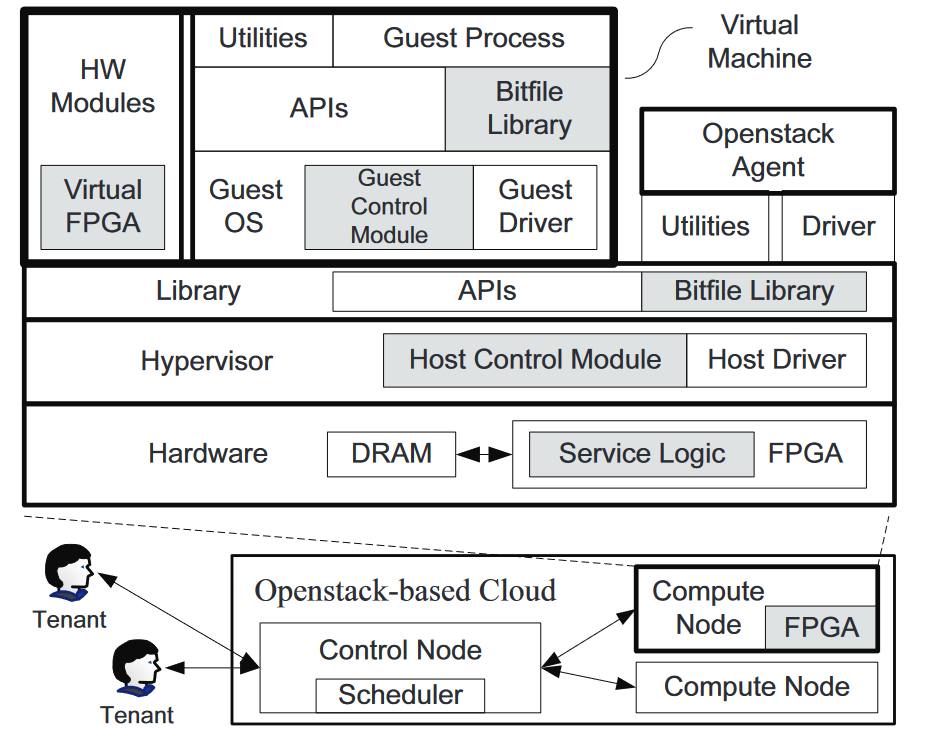
\includegraphics[width=0.8\textwidth]{chen_enabling_architecture.png}
    \caption[Cloud FPGA Architecture]{Cloud FPGA Architecture \cite{chen_enabling_2014}.}
    \label{fig:chen_enabling_architecture}
\end{figure}



\section{Cloud FPGA Security}\label{sec:cloudFPGASecurity}
Two recent works, \cite{jin_security_2020} and \cite{turan_trust_2020} have conducted comprehensive surveys of the state security in cloud based FPGAs. In \cite{jin_security_2020}, the authors discuss several avenues by which multi-tenant FPGAs present new vulnerabilities for FPGA compromise. Additionally, they present a number of solutions for access control in a multi-tenant environment. One such suggestion is the inclusion of a Secure Authentication Module (SAM), which enables verification of each IP by means of a challenge-response protocol. The work does not go into detail about this implementation, but one potential for SAM implementation is Xilinx and Silex Insight's Hardware Security Module (HSM), which facilitates secure key storage and management, as well as a cryptographic engine that could be harnessed for the secure key storage.

The authors of \cite{jin_security_2020} also discuss efforts investigating a novel method of mitigating the other primary concern of a co-tenant FPGA: side channel attacks. As the presence of malicious tenants fully under their own control (as opposed to reliant on an obscured trigger) poses a much higher threat, additional safeguards are needed to limit the amount of information that can be gained from the traditional side channels. One key vulnerability they focus on is power draw. To mitigate the extraction of data through the power side channel, they discuss research that proposes actively injecting noise into power traces, as well as attempting to actively adjust power draw to produce a constant consumption rate regardless of the needs of the functional logic.

The authors of \cite{turan_trust_2020} similarly surveys a wide body of research in the area of cloud computing. One particularly noteworthy idea they present is a research effort that attempts to provide authenticity to a bitstream by associating it with an accompanying software application, which runs on the CPU. In this model, the secure software is responsible for decrypting and programming the bitstream, providing the opportunity for suppliers to ensure that the bitstream is not compromised.

Similar to the efforts discussed previously in this section, \cite{turan_trust_2020} also presents an effort to facilitate the secure implementation of Multi-Tenant FPGAs. Specifically, they discuss an effort wherein a specific FPGA can be provided from a trusted vendor with a pair of asymmetric keys pre-configured, such that the integrator can provide the public key to IP providers to encrypt their bitstreams. In this way, no substantial storage overhead or complex key negotiation effort is required at the time of reconfiguration.

\section{Multi-Tenant Cloud Based FPGA Implementation in Literature}\label{sec:LitImpl}
In ``Cryptographically Secure Multi-Tenant Provisioning of FPGAs''\cite{bag_cryptographically_2020} Bag et al. outline a comprehensive architecture for the implementation of a cloud-compatible FPGA architecture, from which much of the work undertaken by this research effort is derived. This work proposes a platform wherein multiple discrete tenants can occupy VFPGA partitions of a larger PFPGA device in a secured environment. In their proposal, they utilize Key Aggregation Cryptography (KAC) to facilitate the encryption of a symmetric (AES) key, which in turn can be used to decrypt tenant bitstreams within their allocated partition. In this implementation, they utilize a single KAC decryption engine at the PFPGA level, which extracts the AES key and furnishes it to individual AES engines at the VFPGA level. The authors claim that by implementing their design in this manner, the only party which the tenant is required to trust is the FPGA Vendor, who provides the public and private keys used by the KAC engine to decrypt the symmetric key. It should be noted that this work is an extension of \cite{chen_enabling_2014}, discussed previously in Section \ref{sec:fpgaCloud}.


\subsection{Implementation Evaluation}\label{subsec:LitEval}
However, this claim is not completely true. By virtue of decrypting the symmetric key at the PFPGA layer, the Cloud Service Provider (CSP) is in possession of both the encrypted bitstream and the symmetric key required to decrypt it. In essence, this is equivalent to them having access to the IP contained within the bitstream itself. Therefore, the tenant must necessarily also trust the CSP, which is not a policy compatible with the security needs of many would-be tenants.Furthermore, the decrypted AES key is stored into memory, which must be isolated. Unfortunately, resolving this concern by isolating this data from the greater PL is not feasible, as there can be only one entry point into the PL from the DDR, which must be shared with all users. However, if trust can be extended to the static partition (through, say, an FPGA Vendor or third-party certified) bitstream, then DMA isolation units can be employed within each partition to prevent malicious access to the decrypted AES key and the bitstream content. This concept is explored in detail later in this work.

Additionally, this implementation allocates a considerable amount of resources to the multiple identical AES decryption cores, which don't actually yield any additional security benefit since the AES key is present at the PFPGA layer alongside the bitstream it encrypts. Furthermore, this implementation requires a predefined number of VFPGAs per PFPGA, which constrains the CSP's ability to adjust the size and number (inversely) of VFPGAs per PFPGA to adapt to demand. This is a significant limitation for CSPs as the field grows, as flexibility in trading VFPGA size for instance count could be highly advantageous in a volatile tenancy environment. This concept also forms one of the key tenants of this research effort, and is explored in great detail in the remainder of this work.                 % INCLUDE: related work
% !TeX root = ../SDonchezThesis.tex

\chapter{Proposed System Architecture}\label{ch:systemArchitecture}

\section{Proposed Design}\label{subsec:Proposal}
The author proposes modifying the implementation proposed by the authors of \cite{bag_cryptographically_2020}, as outlined in Chapter \ref{ch:relatedWork} to eliminate the need for trust in the CSP, along with eliminating the duplication of the AES IP. To achieve this goal, the author proposes the implementation of an attestably secured partition within the PFPGA fabric, which contains both the KAC and AES engines. By isolating both of these components in an attestably secure partition, the CSP no longer has access to the decrypted symmetric key, preventing them from decrypting the bitstream and gaining access to the IP contained therein. Meanwhile, the presence of the single AES IP in this secured partition eliminates the need for identical engines on each partition, which increases available space and also offers flexibility with regards to VFPGA provisioning, as the only fixed limit remaining is the number of VFPGA device IDs allocated by the FPGA Vendor for the device. This number can simply be made arbitrarily large relative to the realistic number of simultaneous tenants that the device can support, such that the CSP is effectively free to divide the PFPGA as they see fit.

% The presence of a secure partition for decryption operations is useless without the ability to securely transport the decrypted data from said partition to the VFPGA in question. The use of the Hard Processor System (HPS), and specifically a Trusted Execution Environment (TEE) implemented therein, could conceivably facilitate the secure transfer of this information between regions of the FPGA without transiting the unsecured outer region of the programable logic. However, implementation of direct connections between partitions and the HPS such as this necessitates will require further investigation, as the mechanics of such an operation are not currently understood by the author. Alternatively, the use of direct memory access could be a route to secure transfer, although assurance must exist to prevent malicious access to the memory regions in question.

The presence of a secure partition for decryption operations is useless without the ability to securely transport the decrypted data from said partition to the VFPGA in question. Such a task is made far more difficult by the fact that the PFPGA only has a single set of physical connections to the physical memory, which must be commonly utilized by all of the partitions. This requires one of several strategies to ensure data integrity. One option would be for the CSP to allocate dedicated Block RAM to each partition and allow access to it only from the decryption partitions and the given tenant partition. However, such a solution would likely be prohibitively expensive, and would still require the data to traverse an untrusted region of the FPGA at some point.

As an alternative, this paper proposes the use of a trusted (provided by either the FPGA vendor or a trusted third party) top level bitstream, incorporating DMA controllers for each partition that are paired with memory isolation technology contained in the trusted top level bitstream in order to prevent co-tenants from accessing each others' data. Such an architecture is captured in Figure \ref{fig:topLevelDesign}, where the memory isolation logic would be implemented at each partition boundary.

\begin{figure}
  \centering
  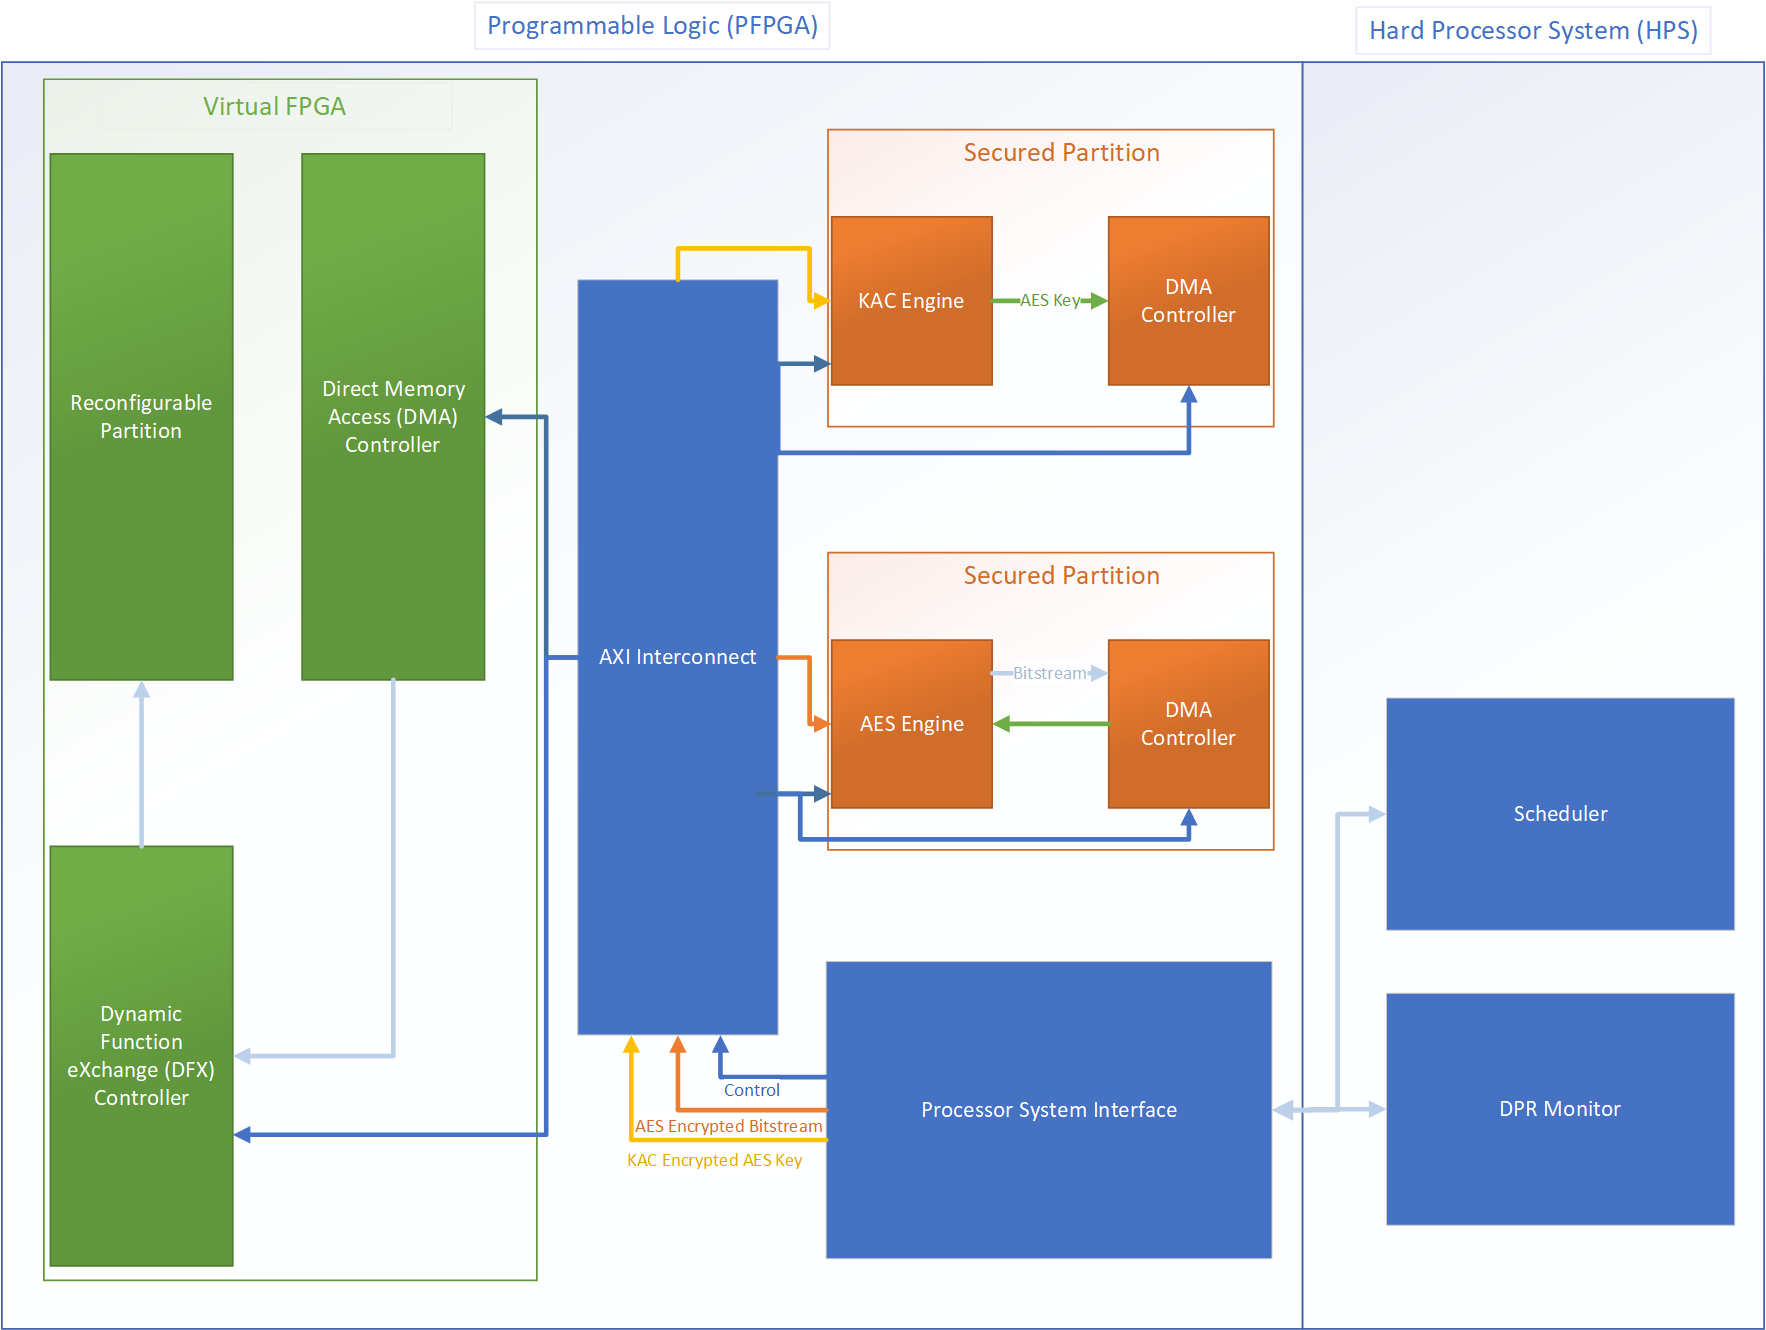
\includegraphics[width=0.8\textwidth]{ConceptDiagramSimplified.png}
  \caption{System Architecture Concept Diagram}
  \label{fig:topLevelDesign}
\end{figure}

The use of the HPS to facilitate such a transfer has additional advantages, as it is conceivable on larger devices that multiple such partitions could be desired to facilitate simultaneous tenant reprogramming. In either case, the use of the HPS to schedule access to the secured partition(s) could similarly prove to be a useful design component.

\section{Architecture Implementation Tasks}\label{subsec:Obj}
The above implementation requires a number of discrete objectives be completed and integrated into a comprehensive design. Those objectives are described below. A subset of these objectives have been evaluated as a part of this research effort, and are described in the subsequent chapters.

\begin{itemize}
  \item Obtain or design the AES and KAC cores for the secured partition.
    \begin{itemize}  
      \item Ideally these cores should be pipelined for efficiency
    \end{itemize}
  \item Investigate direct communication between partition and HPS (without untrusted transit)
  \item Investigate use of DMA to facilitate secure communication between partitions securely
  \item Design and Implement scheduling algorithm to allocate decryption partition to tenants
    \begin{itemize}
      \item With multiple AES cores, it may make sense to share a single KAC engine if secured link between them can be guaranteed (the KAC has to decrypt a single key of trivial size, whereas the AES engine is in much higher demand due to need to decrypt entire bitstream)
    \end{itemize}
  \item Implement attestably secure partition and provide mechanism for attestation and verification
  \item Implement Trusted Execution Environment (if using HPS for secured data transfer)
  \item Implement data routing and verification logic within TEE (if using HPS for secured data transfer)
  \end{itemize}          % INCLUDE: system architecture

% !TeX root = ../SDonchezThesis.tex

\chapter{Decryption Core Scheduling Engine}\label{ch:edfScheduling}

Since the AES engine is decrypting a bitstream, as opposed to a simple key (as is the case in the KAC engine), it will necessarily be occupied for a considerably longer period of time than the KAC engine for each reconfiguration cycle. Furthermore, since the trend in cloud infrastructure is to implement large devices with many partitions rather than many smaller ones, it is likely that a single AES engine per PFPGA will be insufficient to accommodate the partial reconfiguration needs of said device's tenants.

To this end, this architecture proposes the implementation of multiple discrete AES cores, each of which may be attached to a partition for the purposes of facilitating a decryption operation as part of the reconfiguration process. This necessitates the scheduling and allocation of these resources in a fashion that takes into account the real-world constraints of the CSP. To this end, this architecture proposes a modified Earliest Deadline First (EDF) scheduling algorithm, to be implemented on the Hard Processor System (HPS) of the heterogenous system. This algorithm, including its assumptions, constraints, and design, is outlined in the following sections.

\section{Background}\label{sec:EDFRelated}

The concept of utilizing an EDF-based algorithm for scheduling in a real-time environment is hardly a novel idea. In fact, this application was first suggested in 1973 by Liu and Layland in \cite{liu_scheduling_1973}. In their work, the authors propose an algorithm by which independent, periodic tasks with hard deadlines and constant execution times can be efficiently scheduled prior to execution as to ensure each executes before its respective deadline. This algorithm is known as the Earliest Deadline First (EDF) scheduling algorithm. As its name suggests, the algorithm is based on the assumption that maximum utilization of a processor can be achieved by scheduling for immediate execution the task with the nearest deadline, provided that the total utilization required to execute all tasks is less than or equal to the processor's capacity.

The various qualifiers present on the word ``task'' in the above statement are critical, as they are largely incompatible with both modern programming paradigms and with the use of EDF to schedule FPGA-based tasks. In fact, the tasks executed in the use case of a CSP provisioning FPGA partitions can be generally characterized as being aperiodic, featuring flexible deadlines, and, potentially, being interdependent. Furthermore, the original EDF algorithm is a static, a priori algorithm, meaning that the task information is known in advance, and that the algorithm precomputes the optimal schedule before execution begins. The algorithm is then incapable of adapting to any modifications of the task information that may occur during the course of the execution.

In the years that have elapsed since Liu and Layland first presented the algorithm., countless modifications have been proposed which address many of these concerns. In \cite{stankovic_deadline_1998}, the application of the EDF algorithm's key principles to real-time environments (wherein the scheduler is employed dynamically at run time as opposed to a priori). Similarly, \cite{spuri_efficient_1994} enhances the EDF algorithm to accurately schedule aperiodic tasks in conjunction with periodic tasks.

A major shift in scheduling came in the early 2000s with the mass popularity of the multi-core processor. Originally the exclusive domain of supercomputers, multi-core processors became a mainstay of personal computing as a means of avoiding the immense thermal loads associated with the increasing frequency of conventional, single core CPUs. As these processors entered enterprise and consumer markets, it became clear that there was a need to efficiently distribute task load across the various cores. In \cite{abeni_edf_2020}, the authors propose modifications to the EDF algorithm to accommodate multiple cores by means of an ``adaptive migration'' algorithm that emphasizes the minimization of unnecessary task migration between cores.

One constant throughout these developments is that in most cases, the EDF algorithm and its derivatives are intended to schedule tasks on a traditional general purpose processor, whether said processor is a small microcontroller or a large multi-core AMD or Intel flagship. The application of such an algorithm to FPGAs has not previously been considered in the literature, as FPGA-based operations are typically conducted in parallel. Fortunately, most of the concepts upon which the EDF algorithm are based are also perfectly applicable to the scheduling of FPGA-based IP cores. The remaining sections of this chapter outline the application of an EDF-derivative algorithm for this use case.

\section{Assumptions}\label{subsec:EDFAssumptions}
The following assumptions are made regarding the implementation of the AES core scheduling process for this architecture:
\begin{itemize}
    \item The time required to decrypt a given partial bitstream increases linearly with a corresponding increase in file size.
    \item The time required to decrypt a given partial bitstream can be approximated into a discrete number of ``time units''.
    \item Deadlines for decryption are made available as tasks are received, and are driven by real world constraints (License Agreements, Pricing Tier, etc.).
    \item The CSP will not allocate more decryption jobs to the PFPGA than can be scheduled within their given deadlines (meaning that the schedulability does not need to be verified).
    \item The time required to switch from processing one bitstream to processing another is both non-trivial and constant.
    \item The act of reading (ingesting) and writing (outputting) bitstream segments to/from the AES engine requires a known, constant time.
    \item The time required for communication between the HPS and the AES core is assumed to be both constant and trivial.
    \item Due to the nature of the environment in which the algorithm is being implemented, it is important to note that tasks are random and likely aperiodic in nature.
\end{itemize}

\section{Constraints}\label{subsec:EDFConstraints}
The implementation outlined in subsequent sections will be subject to the following set of design constraints, imposed by the assumptions listed in the preceding section as well as best practices:
\begin{itemize}
    \item In the event of a tie between two task for the next time unit, where one task is the task that was operated on in the previous time unit, the task which was previously being executed shall continue to be executed, in order to eliminate overhead associated with context switching between tasks.
    \item As the IP core currently selected for performing the AES decryption operation is non-pipelined, and therefore not capable of transitioning seamlessly between decryption operations without first having its state machine reset, there shall be a small reset delay during context switches
    \item The algorithm shall be implemented for an abstract number of AES cores N, with the assumption that N shall be some small number in the real-world implementation.
    \item The HPS shall communicate with the AES cores via the AXI bus.
    \item The bitstream shall reside in the domain of the PS for purposes of this algorithm, and shall be transferred via the AXI bus.
    \item The atomic unit of the bitstream shall be considered sufficiently large, as too small of an atomic unit will cause scheduling computations to take longer than the time unit itself.
    \item Tasks are placed in a queue, Q, arranged by deadline in ascending order (such that the earliest deadline is at the start of the queue). 
    \item The deadline associated with a processor is the deadline of the task it is currently executing, or $\infty$ if it is idle.
\end{itemize}

\section{Proposed Scheduling Algorithm}\label{subsec:AlgoImpl}[ht!]
Algorithm \ref{alg:EDFAES} implements the scheduling routine for the AES Cores, as governed by the constraints and assumptions outlined above. This algorithm serves as the guidance for the implementation of the Scheduler as outlined in subsequent sections, subject to the constraints and assumptions outlined above.
\begin{algorithm}
    \caption{Global EDF Scheduling Algorithm for AES Decryption Cores}\label{alg:EDFAES}
    \begin{algorithmic}

        %define foreach since it isn't included
        % \algnewcommand\algorithmicforeach{\textbf{for each}}
        % \algdef{S}[FOR]{ForEach}[1]{\algorithmicforeach\ #1\ \algorithmicdo}
        % \algnewcommand\algorithmicendforeach{\textbf{end for each}}
        % \algdef{E}[FOR]{EndForEach}[1]{\algorithmicendforeach\ #1\ \algorithmicend}
        \State We consider a task set $\uptau$ consisting of $x$ tasks $T_1$ , . . . , $T_n$ that are sporadically released from the CSP with arbitrary deadlines
        \State Variables: 
        \State N - the set of cores to be utilized
        \State Q - the queue containing all tasks currently pending execution
        \State $T_{n_i}$ - the task assigned to a given core
        \State $D_t$ - the delay associated with a given task
        \State $D_{n_i}$ - the delay associated with the task currently executing on a core (for brevity)
        \State $D_{Q_i}$ - the delay associated with the task at a given position in the queue (for brevity)

        \\

        \Require $n(N) > 0$ \Comment{There are a nonzero number of cores}

        \Function{SwapTaskToQueue}{$T$}
            \ForAll {$Q_i \in Q$} 
                \If{$D_T < D_{Q_I}$}
                    \State Insert $T$ into $Q$ at index $Q_i$
                    \State \Return pop($Q$)
                \EndIf
            \EndFor
            \State Append $T$ to the end of $Q$ \Comment{If all currently queued tasks expire before $T$}
        \EndFunction

        \\

        \While{true} \Comment{Each Time Unit}
            \ForAll {$n_i \in N $}
                \If{$Q \neq \emptyset$}
                    \If{$D_{n_i} == \infty$}
                        \State $T_{n_i} \gets T_{Q_0}$ \Comment{Pop $Q$}

                    \\
                    \State \Comment {\parbox[t]{.75\linewidth}{If the currently executing task has a later deadline than the first task in the queue and has the latest deadline of any currently executing task across all cores.}}
                    \\

                    \ElsIf{$(D_{n_i} > D_{Q_0})$ AND $D_{n_i} == max(D_N)$}  
                        \State $T_{n_i} \gets $SwapTaskToQueue($T_{n_i}$)
                    \Else
                        \State $T_{n_i} \gets T_{n_i}$
                    \EndIf
                \EndIf
            \EndFor
        \EndWhile
    \end{algorithmic}
\end{algorithm}

It should be noted that, by virtue of comparing the deadline of the first task in the queue against the latest deadline of all currently executing tasks, this algorithm supports preemption. Such a consideration is critical for the success of a scheduler dealing with tasks of varied size, as otherwise a large but long-lead task could cause a short, more urgent task to miss its deadline when both could have been scheduled effectively.

\subsection{Task Model}\label{subsec:TaskModel}
The algorithm outlined in Algorithm \ref{alg:EDFAES} centers around the notion of a task, which is representative of a tenant bitstream that is to be decrypted. From the perspective of the scheduler itself, the task does not necessarily contain this bitstream, as the scheduler is not concerned with the contents of the PL. Rather, the scheduler is provided only with metadata about the task, such as is necessary to schedule it for execution. The following information is stored in this task model:

\begin{itemize}
    \item A Unique ID (arbitrarily constructed) used to refer to the task
    \item A ``human-readable'' name for the task
    \item The number of discrete Time Units of execution the task requires for decryption
    \item The task's deadline
    \item The period of the task, represented as zero if the task is aperiodic
\end{itemize}
In the implementation described below, this information is contained in a JSON structure. Other encoding schemes are certainly feasible, and the software as implemented also supports XML formats when compiled appropriately. An example of a task model is given in the listing below.

\begin{lstlisting}[language=json, caption={An example task object, presented in JSON}, captionpos=b, float]
{
    "deadline": 15,
    "unitsToExecute": 5,
    "taskId": 1,
    "taskName": "Task 1",
    "period": 20
}
\end{lstlisting}

\section{Algorithm Implementation}\label{sec:Impl}

This effort implemented the above algorithm in a test application which is representative of its implementation in the real-world use case outlined in Chapter \ref{ch:systemArchitecture}. However, as the scope of the research completed to date does not include the larger system outlined in that section, it is somewhat constrained with regards to its external interfaces. Namely, it does not attempt to directly affect any actual IP Cores, but rather performs theoretical scheduling of the cores and notes its results in a log file. It does, however, attempt to mimic the likely real-world method of input, in that it parses serialized data such as would be suitable for transmission by a discrete centralized controller overseeing a number of PFPGA instances.

Along with the development of the Scheduler itself, it was also necessary to thoroughly exercise the application to ensure that it functions successfully under load. As a result, it was also necessary to develop a Testbench application, which is capable of generating arbitrary tasks for the AES cores to schedule. This Testbench is capable of generating tasks in accordance with a given target utilization rate. A comprehensive set of interprocess communication (IPC) calls enable synchronization between the two applications. For purposes of ensuring low resource utilization, as well as promoting well organized source code, both of these applications were developed in C++, utilizing an object-oriented approach. Section \ref{subsec:SchedulerImpl}, below, outlines the implementation of the Scheduler itself, while Section \ref{subsec:TestbenchImpl} outlines the implementation of the Testbench. Section \ref{subsec:IPC} outlines the interconnection of these two applications.

\subsection{Scheduler Implementation}\label{subsec:SchedulerImpl}
The Scheduler application consists of several interrelated threads operating in parallel. First among these is an input parser, which waits for serialized task information and, upon receipt, deserializes it into task objects. For the sake of best practices (as well as ease of parsing), this data is encapsulated in a JavaScript Object Notation (JSON) string, which, despite its name, is a language agnostic structure that is commonly used to represent entities. In its current implementation this data is simply read from a file descriptor (such as standard input), although future extensibility to a socket based architecture for network communications is possible.

Alongside the input parser is the timer manager. The timer manager is responsible for managing the discrete units of time for which the cores can be scheduled. The AES cores intended for use in the larger research effort are currently non-pipelined cores requiring a fixed number of clock cycles to process each word of data. Accordingly, the frequency with which they can be scheduled is based on a multiple of that number of clock cycles, which must be small enough to afford flexibility but high enough to minimize wasted cost due to context switching (per the design assumptions). As the HPS and the PL do not necessarily share a common clock, and as the execution of the various threads on the processor is non-deterministic in its own scheduling, it is necessary to utilize a timer to ensure scheduling operations are executed exactly once per atomic unit of IP Core schedulability. This thread provides that functionality, and sets flags for the other threads as needed to facilitate their operation.

The final (and arguably most consequential) thread of the Scheduler application is the core servicer itself, which is responsible for ensuring each core is executing the ideal task per the prescribed algorithm. Once per Time Unit, the core servicer evaluates the deadlines of the tasks currently executing on the cores against those contained in the Scheduler's Task Queue, and performs substitutions as necessary to ensure that the tasks with the nearest deadlines are those currently in execution. 

For purposes of this effort, these services are implemented using C++'s standard threading library (as opposed to the more traditional ``pthread'' library). This threading implementation was chosen to promote cross-platform interoperability, as well as performance optimization where possible.


\subsection{Testbench Implementation}\label{subsec:TestbenchImpl}
The Testbench application in in many ways appreciably simpler than the Scheduler itself. It is only a single threaded application, and the task it performs is straightforward - it simply creates tasks populated with arbitrary information. However, this seemingly straightforward operation is greatly complicated by one of the assumptions outlined in Section \ref{subsec:EDFAssumptions} above. Namely it is the fourth assumption in that section which proves problematic: The CSP will not allocate more decryption jobs to the PFPGA than can be scheduled within their given deadlines. This greatly eased the development of the Scheduler itself, by eliminating the need for it to perform schedulability checks as part of its task processing. However, as the Testbench is effectively serving as the CSP in these simulations, it falls to the Testbench to ensure that the tasks it generates do not overload the PFPGA instance for which the Scheduler is allocating resources.

This is accomplished through introducing some element of reporting to the Scheduler itself, and making those results available to the Testbench. Specifically, the Scheduler maintains a table outlining how many outstanding time units need to be executed by any given point in time, as described by the sum of all of the outstanding units for each task due at that point. By combining this information with knowledge of what unit in time the PFPGA and PS are currently in, it is possible to validate in real time the schedulability of a task as it is being generated, and to make adjustments as needed. 

This logic is captured in Equation \ref{equ:Utilization}, below. In this equation, $t_c$ represents the current Time Unit, $t_n$ represents the time unit being proposed as the deadline for the task, $D_i$ represents the number of units due at time $i$, and $UtE$ represents the number of Units to Execute for the task currently being evaluated. $P$ is the parallelization factor, or the number of cores which the schedule is being distributed between, while $n-c$ yields the total number of TimeUnits between the time the equation is evaluated and when the deadline will come. The ``Desired Load Percentage'' is the target utilization rate for the cores.

\begin{equation}\label{equ:Utilization}
    \frac{(\sum_{i=t_c}^{t_n}D_i)+UtE}{P*(n-c)} < Desired\:Load\:Percentage
\end{equation}

By verifying the validity of this equation for each generated task's proposed deadline, it is possible to ensure that target average utilization is not exceeded. Furthermore, the maintenance of this information on the part of the Scheduler is non-resource intensive, requiring a single addition operation as each task is parsed, a single decrement operation as each core is serviced, and a single increment operation (for the current unit counter) on the part of timer manager per Time Unit.

Unfortunately, this does not fully resolve the issue outlined above. In addition to ensuring that the average utilization is not compromised, it is also important to verify that the instantaneous utilization never exceeds the maximum. (For example, inserting a task that has a Units to Execute value of 100 with a deadline of 500 may not compromise the average utilization, but may cause a task due at unit 510 to lack sufficient time to run). To rectify this, an additional check is necessary. 

To perform this additional check, the generator iterates across the entire simulation window, computing a running sum of the outstanding work to be done that is due at that unit, and comparing that value plus a prorated portion of the new task's units against the theoretical limit. This check is captured by Equation \ref{equ:InstUtil}:
\begin{equation}\label{equ:InstUtil}
    \sum_{i=t_0}^{t_n}D_i + \max(\min(UtE, i - t_c), 0) < P*(n-i-c)\:\forall i>c
\end{equation}

Provided the conditions of both Equations \ref{equ:Utilization} and \ref{equ:InstUtil}, above, are satisfied, the Testbench application can then assume that the proposed deadline is valid for the generated task.

\subsection{InterProcess Communications}\label{subsec:IPC}
The inclusion of an operating system into this research effort greatly eased efforts to facilitate communication between the two discrete applications. Both Windows and Linux implement comprehensive facilities for InterProcess Communication (IPC), which enable the transfer of data between applications. Unfortunately, the two systems do not have a common set of IPC functions, requiring slightly difference implementations to satisfy the two architectures. Despite this, the overall design of the IPC structures for the two architectures is effectively the same.

\subsubsection{Testbench to Scheduler Communication}\label{subsubsec:TestbenchSchedIPC}
Communication from the Testbench application to the Scheduler application is straightforward, as the only traffic flowing in this direction is the serialized task data. Since this data is serialized and relatively small in size, and in the interest of replicating the real-world functionality of the software, this data is simply read in from a file descriptor. In Windows, this is accomplished via a Named Pipe, which effectively enables the data to be consumed as if it were typed into the standard input of the application in the terminal window in which it is executing. Specifically, this named pipe was configured in ``message'' mode, such that the entire task is treated as an atomic unit for purposes of the transfer, rather than its constituent bytes (the latter configuration can result in multiple or even partial messages being sent as a single input, which would unnecessarily complicate the parsing operation).

Linux also provides a ``Named Pipe'' functionality, but this functionality is strictly byte-oriented as opposed to message-based. Accordingly, it is not desirable for use in this scenario. Fortunately, the Linux system also supports System-V Message Queues, a part of the Posix standard that is functionally equivalent to Windows's Named Pipes in message mode. The only impactful difference between the Windows and Linux implementations of this facility is that the Linux implementation does not facilitate the ability to wait for a connection, thus requiring the use of a Semaphore (another POSIX IPC method) to ensure synchronization between the two applications.

\subsubsection{Scheduler to Testbench Communication}\label{subsubsec:SchedTestbenchIPC}
The transfer of data from the Scheduler to the Testbench is appreciably more complex, as the table of Outstanding Units Due (used in Equation \ref{equ:Utilization}) is updated during each TimeUnit, and contains $P*N$ words of data, where N is the number of time units to simulate and P is the number of IP Cores. It would be inefficient to the point of impracticability to transfer and parse that data every time unit, as its scale for even modest simulations would likely consume a non-trivial portion of the available compute time to parse. Accordingly, the implementation instead uses a shared memory space for the purposes of facilitating this communication, accomplished in Windows by utilizing the File Mapping functionality of the Win32 API, and in Linux via the comparable Shared Memory Segment functionality. In this way, the generator simply receives a pointer to the Scheduler's own copy of the table, and is always able to view the latest updates to it without any need for direct transfer between the applications.

The same functionality is utilized for the mapping of the current Time Unit between the two systems, as it eliminates any edge cases wherein the unit changes shortly after the Testbench queries it. This allows for the most accurate possible scheduling of tasks.

\section{Development and Test Environment}\label{sec:environment}
The implementation above utilized a number of development tools and platforms, and targets a specific set of hardware and supporting software as outlined in the following subsections. While it may (and likely will) execute under other conditions, the performance of the algorithm cannot be guaranteed outside of the specified test environment.

\subsection{Target Hardware}\label{subsec:targetHW}
The Scheduler and testbench implemented in \ref{sec:Impl} target the AVNet ZedBoard Development Board. The ZedBoard contains a Xilinx XC7Z020-CLG484-1 heterogenous SoC, featuring a Dual-Core AR Cortex-A9 MPCore processor and an Artix-7 series FPGA with 85,000 logic cells. The board also features 512MB of DDR3 memory, 256Mb ofQuadSPI Flash memory, and a 10/100/1000 Ethernet Interface. It also has integrated JTAG and PS UART interfaces, which greatly simplifies the loading and debugging of the applications and bitstreams used in the testing process. A diagram of the ZedBoard, with key I/O connections indicated, is provided in Figure \ref{fig:zedImg}.

\begin{figure}[ht]
    \centering
    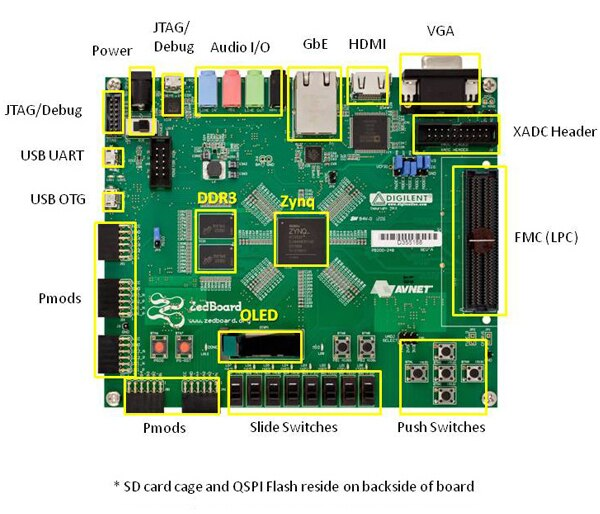
\includegraphics[width=0.8\textwidth]{ZedBoard-Overlay.jpg}
    \caption[ZedBoard Schematic]{ZedBoard Schematic, with key I/O \cite{noauthor_zedboard_nodate}.}
    \label{fig:zedImg}
\end{figure}

For purposes of evaluating the performance of the scheduler implementation, the PL of the ZedBoard was loaded with AVNet's stock reference design, which instantiates the PS-PL interfaces, the DDR3 controller, and the various General Purpose Input Output (GPIO) modules. This design is depicted in Figure \ref{fig:zedGPIODesign}. More robust implementation of the scheduler such as would be suited for full integration into the architecture developed in Chapter \ref{ch:systemArchitecture} would require the use of a customized design. Figure \ref{fig:zedResourceConsumption} provides statistical data demonstrating the resource utilization associated with this design. As is clear from the data, the ZedBoard's resources are more than ample for this simple design, despite its age. That being said, the implementation of multiple AES (and KAC) cores would likely tax its resources such that it would be unsuitable for use. Consequently, further research efforts seeking to fully implement the entire architecture proposed in Chapter \ref{ch:systemArchitecture} would likely need a more modern, larger FPGA.

\begin{figure}
    \centering
    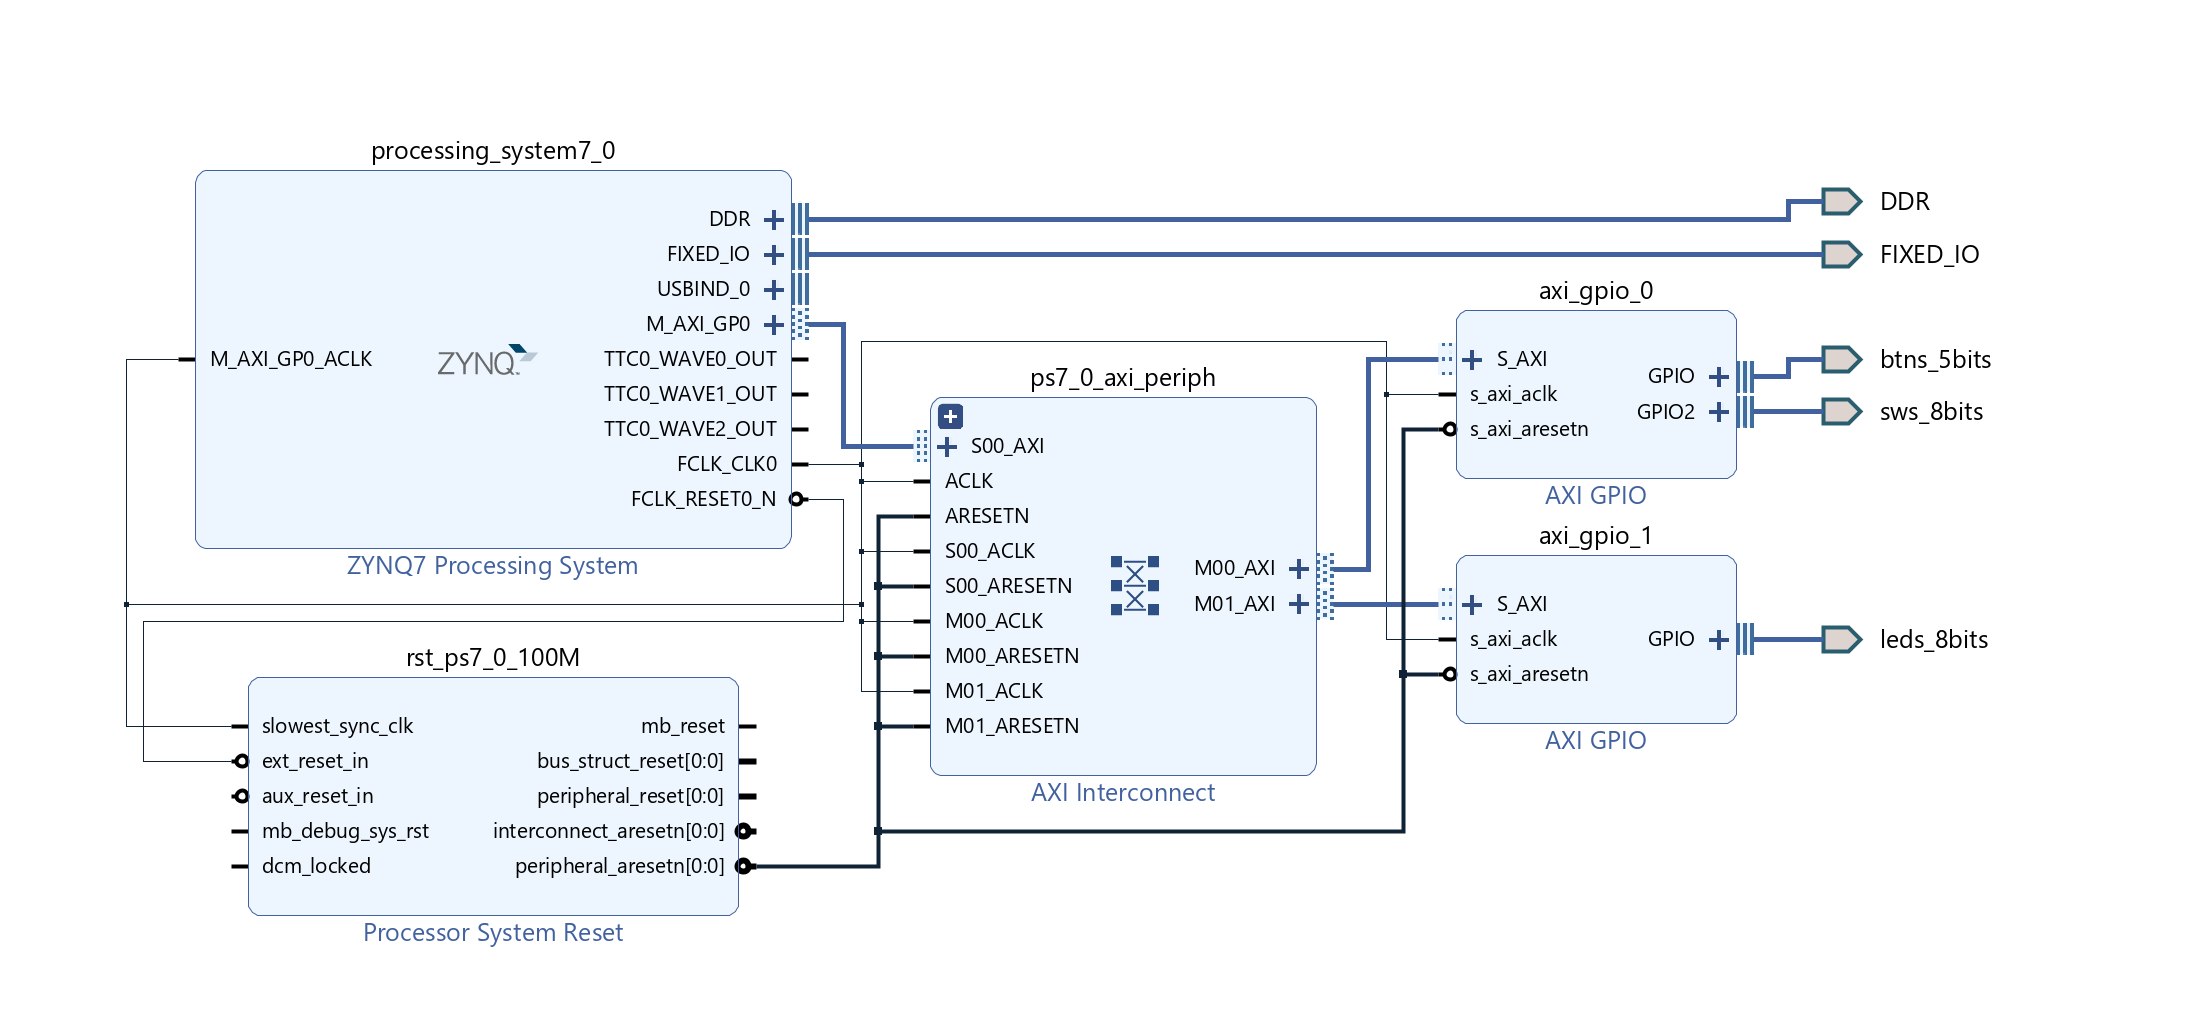
\includegraphics[width=0.8\textwidth]{zed_hw_gpio_bd.png}
    \caption[ZedBoard Reference Design]{Block Diagram of the ZedBoard Reference Design}
    \label{fig:zedGPIODesign}
\end{figure}

%TODO: Add screenshot of PS Interface config - indicate that there is work involved

\begin{figure}
    \centering
    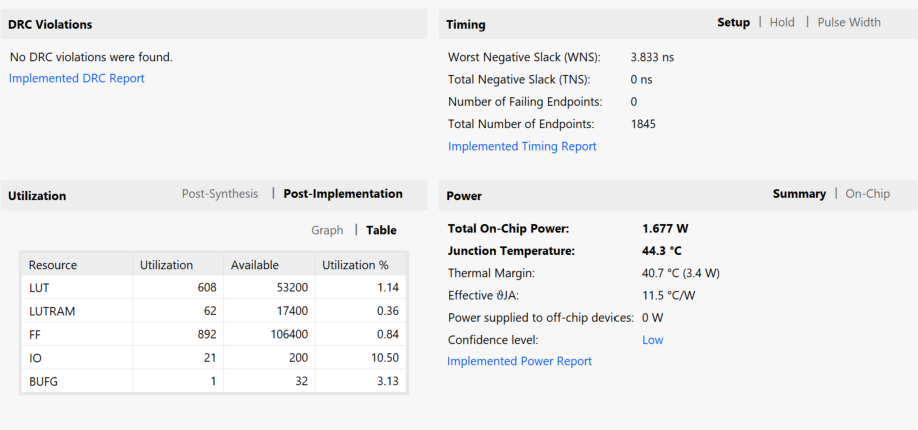
\includegraphics[width=0.8\textwidth]{zed_hw_gpio_stats.png}
    \caption[ZedBoard Resource Consumption]{ZedBoard Resource Consumption}
    \label{fig:zedResourceConsumption}
\end{figure}

\subsection{Target Operating System}\label{subsec:os}
By virtue of introducing multiple threads to the scheduler (and also by virtue of running two applications on a single core processor), it is necessary to implement an operating system (OS) on the processor system upon which the scheduler simulation is running. Futhermore, the larger design will add additional functionality to the processor system, further necessitating an operating system for thread management and for scheduling of the processor itself. To this end, several operating system choices were considered for implementation on the hardware target in support of this simulation. As the target in question includes a Xilinx SoC, it was decided that the ideal choice for such a system would be the Xilinx PetaLinux OS, as it includes all of the necessary drivers for interfacing with the various devices on the development platform. Additionally, the PetaLinux platform is based on the OpenEmbedded Project's toolchain, which affords tremendous flexibility and customization potential as needed. For purposes of this effort, PetaLinux 2020.2 was chosen for compatibility with the equivalent versions of the Xilinx design tools (discussed in Subsection \ref{subsec:devEnv}, below) already in use. This PetaLinux version is derived from Linux kernel version 5.4.

For ease of development and testing, the two software applications were designed to run both in the native Windows environment of the development computer as well as the Linux environment of the target. This reduced cycle time between incremental iterations of the applications, as well as eliminated dependence on an extensive physical setup for testing.

\subsection{Development Environment}\label{subsec:devEnv}
Although the hardware specifications of a development machine are of little consequence to the implementation itself, they are provided here for sake of completeness and perspective to those attempting to replicate the results. The development machine used by the authors in the course of this project was a Windows 10 Professional Edition 64-bit laptop featuring an Intel Core i7-9750H CPU with a base frequency of 2.60GHz. The machine featured 16 GB of DDR4 DRAM and a 1 TB SSD.

The scheduler and testbench applications were first developed for Windows to ease testing, and then later ported to the hardware target. For Windows development, the author utilized Visual Studio 2019 Enterprise Edition, which is available to students free of charge through Microsoft's Azure for Students program. It should be noted, however, that the enhanced feature set of the enterprise edition was not strictly necessary, and that implementation and compilation using the community edition (which is free of charge to all users) is certainly possible.

The construction of the PetaLinux operating environment outlined in \ref{subsec:os} requires a linux environment. To this end, the author constructed a Docker container based on the ubuntu:18.04 image, and extended with the full Xilinx 2020.2 toolchain (Vivado, Vitis, and the PetaLinux toolchain). The container was used for all stages of the linux port and implementation, from hardware export to operating system implementation to application compilation. The container was wrapped in a Visual Studio Code devcontainer, a Microsoft concept that automates the construction of docker images and integrates them into the Visual Studio Code ecosystem, for sake of convenience. The container specification is provided in appendix \ref{apx:EDFDocker} for guidance. Note that users will need to provide their own Xilinx installers and license files.

\section{Experimental Results and Discussion}\label{sec:findings}
The implementation of the EDF algorithm and Testbench on the Windows target has revealed that it is able to successfully schedule tasks at high utilization levels with low miss rates, given that the requirements outlined in the design constraints and assumptions are met. Careful analysis of the Scheduler's output reveals that it is scheduling in accordance with the algorithm, with only a single exception - at the end of the simulation, as the task queue depletes, the Scheduler unnecessarily shifts tasks from higher index cores to vacant lower-indexed cores. Ultimately, this inconsistency is non-consequential, as in a real-world implementation it is unlikely that the task queue would ever be depleted (and also as it does not cause any tasks to miss their deadline).

\subsection{Scheduler Effectiveness at Varying Utilization Levels}\label{subsec:SchedulerDataUtilVary}
As the primary measure of success for this Scheduler implementation is how it performs under heavy load, a series of trials were conducted on the hardware target under varying levels of load in order to determine the average performance of the algorithm for each loading. These results are described in Table \ref{table:SchedEffectivenessUtilVary}, below. All iterations were performed for a simulation of 1000 TimeUnits, with the number of decryption cores fixed at 4. The results below are computed from the average of three trials for each utilization, each utilizing a different randomly generated set of tasks.

\begin{table}[ht!]
    \centering\begin{tabular}{| c | c | c | c |}
        \hline
        Target Utilization & Number of Tasks & Units Elapsed & \% Units Missed \\
        \hline
        50\% & 38 & 512 & 0\% \\
        60\% & 47 & 604 & 0\% \\
        70\% & 53 & 732 & 0\% \\
        80\% & 64 & 825 & 0\% \\
        90\% & 74 & 925 & 0.15\% \\
        100\% & 82 & 1000 & 8.63\% \\
        \hline
    \end{tabular}
    \caption{Scheduler effectiveness at varying utilization with fixed core count}
    \label{table:SchedEffectivenessUtilVary}
\end{table}

These findings indicate a high level of success on the part of the scheduling algorithm, as it effectively schedules tasks even at high levels of utilization. It is worth noting that the case of 100\% utilization is a special case, as a detailed analysis of individual runs reveals some discrepancies that explain the high miss rate. The current implementation of the Testbench does not immediately send a task at TimeUnit = 0 on every iteration, as its operation is, by design, random. As a result, the logged allocation of cores to tasks often indicates empty cores for the first several TimeUnits. However, the Testbench is still attempting to generate 100\% of the TimeUnits (4000 in the case of these trials), meaning that it will occasionally overschedule the processor. It has been observed through additional experimentation that the increase in miss rate between 90\% and 100\% utilization more nearly approximates an exponential line of best fit than a linear one, further validating the performance of the algorithm.

\subsection{Performance Evaluation at Varying Utilization Levels}\label{subsec:performanceDataUtilVary}
Although the effectiveness of the algorithm (and its implementation) are by far the most important criteria for evaluating their success, it is also important to consider the performance of the application. In the context of the larger system outlined in Chapter \ref{ch:systemArchitecture}, a number of other processes will likely have to execute on the single core available on the hardware target. Accordingly, it is crucial that the Scheduler is not overtaxing the HPS, such that the other portions of the system are also able to execute as needed. Accordingly, Table \ref{table:SchedPerfUtilVary}, below, reports on the total utilization time of the processor for each of the iterations above.

\begin{table}[ht!]
    \centering\begin{tabular}{| c | c | c | c | c |}
        \hline
        Utilization & Clock Time & User Time & System Time & RAM Used \\
        \hline
        50\% & 10.79s & 10.34s & 0.07s & 10.48MB \\
        60\% & 11.04s & 10.35s & 0.06s & 10.63MB \\
        70\% & 10.85s & 10.35s & 0.07s & 10.61MB \\
        80\% & 10.93s & 10.33s & 0.11s & 10.54MB \\
        90\% & 10.87s & 10.39s & 0.05s & 10.73MB \\
        100\% & 10.92s & 10.39s & 0.09s & 10.63MB \\
        \hline
    \end{tabular}
    \caption{Scheduler performance at varying utilization with fixed core count}
    \label{table:SchedPerfUtilVary}
\end{table}

As is evidenced in the table, Resource consumption is not closely correlated with target utilization, but appears roughly constant across all target utilization levels. This is highly beneficial in this scenario, as, with the larger and more complex Task data that will necessarily accompany real tasks being implemented on real IP, any utilization correlated growth in resource consumption would be greatly magnified (and as it is desireable to maximize utilization for revenue purposes on the part of the service provider). 

It should also be noted that much of the ``User Time'' listed in Table \ref{table:SchedPerfUtilVary} above is currently ``idle'' time. As the current implementation of the Scheduler is not controlling real IP, most of the time in each TimeUnit is spent waiting for the unit to expire. This waiting process is not optimized to minimize processor consumption in the implementation used to generate these results, as it is a placeholder for future work.

\subsection{Scheduler Effectiveness at Varying Core Counts}\label{subsec:SchedulerDataCoresVary}
In addition to understanding how the scheduler behaves under varying utilization levels, it is also critical to ensure that it works across a range of core counts. Accordingly, the scheduler was exercised at a fixed load percentage (75\%) for several trials at core counts ranging from 1 to 5 in order to further characterize the performance of the algorithm. These results are captured in Table \ref{table:SchedEffectivenessCoresVary}, below.

\begin{table}[ht!]
    \centering\begin{tabular}{| c | c | c | c |}
        \hline
        Number of Cores & Number of Tasks & Units Elapsed & \% Units Missed \\
        \hline
        1 & 15.33 & 719.67 & 0.00\% \\
        2 & 29.00 & 737.00 & 0.00\% \\
        3 & 43.67 & 774.00 & 0.55\% \\
        4 & 59.33 & 777.67 & 0.12\% \\
        5 & 79.33 & 778.00 & 0.00\% \\
        \hline
    \end{tabular}
    \caption{Scheduler effectiveness at varying core count with fixed utilization}
    \label{table:SchedEffectivenessCoresVary}
\end{table}

As can be seen here, an increase in the number of cores causes the testbench to output a proportionally larger number of tasks, although the correlation is not precise due to variations in task length (as the testbench is attempting to meet a target number of TimeUnits, not a specific task count). Furthermore, there does not appear to be a strong correlation between the number of cores and the miss rate of the scheduler, which is an critical indicator of scalability. Were there to be positive correlation, it would indicate that CSPs may have difficulty implementing such a scheme on the larger PLs that would be preferable to operate in a datacenter, as these would require a higher number of cores to service their various partitions.

\subsection{Performance Evaluation at Varying Core Counts}\label{subsec:performanceDataCoresVary}
As with the case of varying utilization levels, it is important to consider scheduler performance from a resource utilization perspective alongside one of pure accuracy, as an accurate scheduler is of limited use if it does not enable the processing system to perform the various other activities required to operate the heterogenous system. The performance characteristics of the implementation against designs with varying numbers of cores is captured in Table \ref{table:SchedPerfCoresVary}, below.

\begin{table}[ht!]
    \centering\begin{tabular}{| c | c | c | c | c |}
        \hline
        Number of Cores & Clock Time & User Time & System Time & RAM Used \\
        \hline
        1 & 11.96s & 10.31s & 0.06s & 10.74MB \\
        2 & 11.14s & 10.35s & 0.05s & 10.67MB \\
        3 & 11.04s & 10.32s & 0.10s & 10.64MB \\
        4 & 10.88s & 10.35s & 0.08s & 10.76MB \\
        5 & 11.12s & 10.38s & 0.06s & 10.67MB \\
        \hline
    \end{tabular}
    \caption{Scheduler performance at varying core count with fixed utilization}
    \label{table:SchedPerfCoresVary}
\end{table}

These results bear remarkable similarity to those discussed in Section \ref{subsec:performanceDataUtilVary}, as evidenced by the lack of correlation between the number of cores and the resource utilization. Although lack of correlation itself is not a positive, lack or correlation in conjunction with low data volatility is indicative of a constant and predictable performance, which is critical for many of the same reasons discussed in Section \ref{subsec:SchedulerDataUtilVary} pertaining to the desire of CSPs to utilize large FPGAs with many partitions and therefore multiple decryption cores.               % INCLUDE: Network DPR
% !TeX root = ../SDonchezThesis.tex

\chapter{Key Aggregate Cryptography}\label{ch:keyAggregateCryptography}
One of the key tenants of the architecture proposed in \cite{bag_cryptographically_2020}, and which is similarly incorporated into this work's architecture, is the use of Key Aggregate Cryptography (KAC) to enable the secure and efficient exchange of encrypted bitstreams between a tenant designer and the CSP. KAC is an asymmetric cryptographic mechanism whereby a single set of public and private ``Master Keys'' can be used in conjunction with a set of ``Aggregate Keys'', each of which affords decryption access to only a subset of the data originally encrypted. In \cite{bag_cryptographically_2020}, the authors utilize this functionality to ensure that only the specific target FPGA can decrypt the tenant bitstream, greatly reducing the scope of vulnerability of the bitstream to third-party compromise.

The concept of Key Aggregation Cryptography is very much a novel area for academic research, having been first proposed in 2013 in \cite{chu_key-aggregate_2014}. The remainder of this chapter will outline the concepts behind KAC based encryption in detail, as well as discuss the use of it in \cite{bag_cryptographically_2020} to facilitate secured bitstream exchange. It will then conclude with the discussion of the cryptosystem within the context of the proposed system architecture, as it relates to the memory isolation functionality discussed in \ref{ch:dmaProtection} as well as with regards to the efficient use of the cryptocore across the various partitions.

\section{Background}\label{sec:KACBackground}
The concept of a Key Aggregate Cryptosystem was first proposed in \cite{chu_key-aggregate_2014} as a means to facilitate the convenient distribution of media assets with targeted access permissions. In today's infrastructure, one could envision its function in a manner similar to Google's Drive storage (or Microsoft's comparable OneDrive). In both instances, a user can upload a set of files, and provide unique permissions on each, thereby enabling only the intended users to access each file. Of course, the technical implementation of these systems does not actually utilize the concept of Key Aggregate Cryptosystems, but the effect is similar.

The implementation of a KAC system is based heavily on ecliptic curve cryptography, a common cryptosystem in widespread use in modern encryption. It is comprised of 5 distinct steps, each of which is discussed below:
\begin{itemize}
    \item \textbf{System Initialization}: The implementer specifies a number of distinct partitions (indices) for the system, as well as a key strength, $\lambda$. $\lambda$ is used to constrain the size of the random data set used to generate the Master Public and Secret Keys, which enable the encryption and decryption of all partitions' data. 
    \item \textbf{Key Generation}: The implemented then specifies (or randomly selects, perhaps programmatically) a random value which is utilized in conjunction with the random dataset (constrained by the $\lambda$ value from the \textit{System Initialization} step) to generate the Master Public and Secret Keys. 
    \item \textbf{Data Encryption}: The data to be encrypted is assigned an index, and is then encrypted using the Master Public Key. The details of the encryption process far exceed the scope of this effort, but generally, given the Master Public Key, the index value, and the data to be encrypted, the engine outputs the ciphertext representative of the data.
    \item \textbf{Partition Key Extraction}: Given a set of indices (which may contain as few as a single index), the extraction functionality generates an Aggregate Secret Key, which is sufficient to decrypt the data associated with the given indices, while not enabling the decryption of any other data. The nature of this process is once again outside the scope of this research effort, but it is important to note that the size of the Aggregate Secret Key is constant, regardless of the number of indices in the set it unlocks.
    \item \textbf{Data Decryption}: Given the Aggregate Secret Key, in conjunction with an index value covered by said key, the decryption process reverses the encryption, yielding the original data. Attempts to decrypt data which is not covered by the Aggregate Secret Key can not only easily be detected, but are mathematically guaranteed to result in a decryption failure.   

\end{itemize}

Figure \ref{fig:KAC_simple} shows a simple example of the KAC process, implemented in the context of encrypting data for shared network storage.

\begin{figure}[ht]
    \centering
    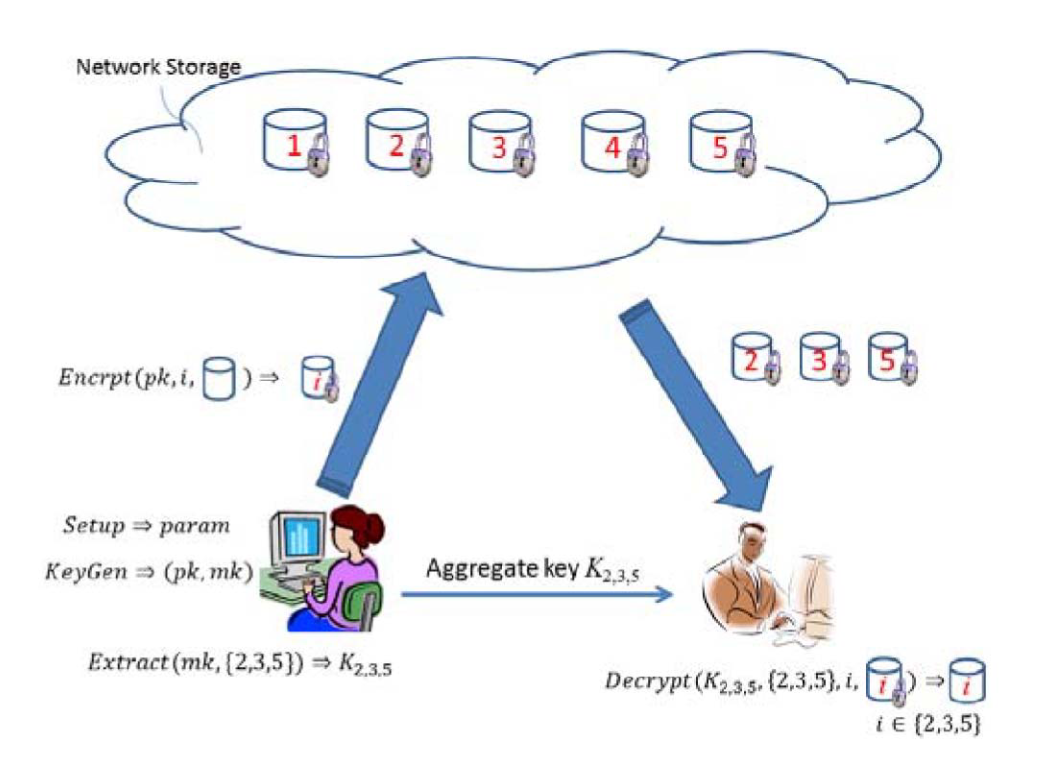
\includegraphics[width=0.7\textwidth]{KAC_simple}
    \caption[KAC Example]{A trivial example of a KAC system in use for network storage. \cite{chu_key-aggregate_2014}}
    \label{fig:KAC_simple}
\end{figure}

An infrastructure such as is afforded by a Key Aggregate Cryptosystem is doubtlessly invaluable for many applications where centralized and easy encryption of data is desired while granularity of access control is still necessary. Although the original developers of the concept in \cite{chu_key-aggregate_2014} present it as a mechanism for facilitating patient access to medical records (and the easy delegation of dependents, etc.), it also has tremendous potential in cloud applications, especially in multi-tenant systems where decryption resources are central and shared. The authors of \cite{bag_cryptographically_2020} implement just such a system in their solution to this design paradigm.

\section{Utilization in Literature}\label{sec:KACLiterature}
The authors of \cite{bag_cryptographically_2020} utilize a hybrid KAC-AES infrastructure to leverage the strengths of both symmetric and asymmetric encryption. KAC, as an ECC derivative, is an asymmetric encryption protocol. Accordingly, different keys are utilized for encryption and decryption operations. This is a tremendous boon from a security perspective in this instance, as the secret key used for decryption need never be provided to tenant designers for encryption. Instead, it can reside in the hardware performing the decryption, likely in isolated memory such as Battery Backed RAM (BBRAM) or Fusible Flash Memory (commonly known as eFUSE in Xilinx devices). In the case of KAC specifically, this strength is enhanced in that the index value must also be known in addition to the secret (aggregate) key, greatly reducing the risk of compromise in the event of secret leakage. However, Asymmetric encryption has its drawbacks, namely that it is a slow and involved process, and is therefore not necessarily well suited to large ciphertext such as a bitstream.

Meanwhile, symmetric encryption (and decryption) offers greatly enhanced performance, and is therefore well suited to large ciphertexts. However, it requires the secure transmission of a common key utilized for both processes, and therefore has inherent security risks. Further, the use of a common key expressly excludes the possibility of a KAC-like segmentation protocol, requiring the use of a separate key for both encryption and decryption of each piece of data.

Bag et. al. in \cite{bag_cryptographically_2020} utilize KAC to transmit a single small ciphertext for each tenant transaction. This ciphertext is associated with a single index value, which correspondingly is matched to the specific tenant partition on which the bitstream is intended to reside. Decryption of this ciphertext (which necessarily occurs in the KAC engine on the target device) yields an AES key. This AES key, in turn, was used by the tenant designer to encrypt the bitstream, using functionality such as is already supported by Xilinx's Vivado tooling and other comparable products. The authors then pass this key to an AES core dedicated to the partition in question, which uses it to decrypt the bitstream and program the partition with the bitstream.

It is easy to see the appeals of this approach, as it enables the secure transfer of the bitstream without relying on complex key-exchange algorithms. It also enables the tenant to specify their own key for bitstream encryption, allowing for easy compliance with any security requirements they may have. Furthermore, the use of KAC has a unique benefit in this environment: only the FPGA vendor, who is entirely uninvolved in the bitstream transfer process, holds the Master Secret Key. It stands to reason that said key can be strictly controlled by said vendor, and thus has a much lower risk of compromise than an aggregate key. (Of course, sensitive applications, such as military use, may choose to replace the FPGA Vendor with their own stringent root-of-trust). Accordingly, any compromised (aggregate) secret key would only be valid for a very small subset of tenants that happen to have targeted that specific hardware instance when encrypting their data, greatly reducing the vulnerable area in the event of such a compromise. 

This design has benefits to the FPGA vendor as well. The FPGA vendor's development tools (as, at least in the current state of the industry, the hardware vendor is also the tool vendor for PL development efforts), which currently are largely configured for user-provided key based symmetric encryption of bitstreams, can remain effectively unchanged, as from the perspective of bitstream encryption this is still the method utilized. Meanwhile, the vendor only needs to distribute a single public key to CSPs, who in turn provide it to tenants. This alleviates them of the burden of complex key management.


\section{Adaptation to Proposed Architecture}\label{sec:KACArchitecture}
The architecture proposed in Chapter \ref{ch:systemArchitecture} does not require massive overhauls to the encryption scheme presented in \cite{bag_cryptographically_2020}. The overall structure of the scheme, whereby a KAC engine decrypts an AES key that in turn is used to decrypt the tenant bitstream, remains intact in this effort's implementation. What changes is the number of AES cored present in the target hardware instance's hardware. In the literature implementation, there is a unique core per partition, hardcoded with that partition's index value as shown in Figure \ref{fig:bag_architecture}. This imposes substantial overhead for large FPGAs, which may have tens (or more) of partitions. 

\begin{figure}[ht]
    \centering
    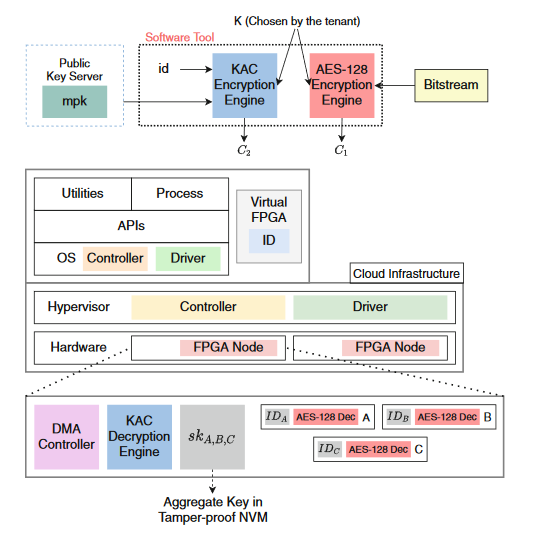
\includegraphics[width=0.6\textwidth]{bag_architecture}
    \caption[Literature Cryptosystem Implementation]{Implementation of a hybrid KAC-AES cryptosystem with one AES core per partition. \cite{bag_cryptographically_2020}}
    \label{fig:bag_architecture}
\end{figure}


In this effort's implementation, the number of AES cores is no longer linearly correlated (although perhaps necessarily proportional) to the number of partitions. Instead, it is assumed that each partition spends the majority of its time not in a state of actively being reconfigured, and therefore it is presumed feasible to share the AES cores among multiple partitions. To this end, the cores (scheduled by the EDF-based scheduler outlined in Chapter \ref{ch:edfScheduling}) are no longer statically assigned index values. Instead, these values are dynamically assigned by the scheduler as the core is assigned to a partition.

Although this mechanism does inject some additional complexity into the decryption process, it actually affords further enhanced security. By dynamically assigning the index value to the core, the capability to decrypt the AES key is no longer simply constrained to a single hardware target, but is in fact constrained to that target only during the period for which the KAC engine is specifically allocated to that partition. As the KAC engine is only decrypting a trivially small ciphertext (the AES key), it will not need to spend much time assigned to any given partition. This fact, coupled with the retention of the decrypted AES key for only as long as is needed to facilitate bitstream decryption, immensely reduces the already small vulnerable surface for bitstream compromise in the event of aggregate key leakage.    % INCLUDE: KAC
% !TeX root = ../SDonchezThesis.tex

\chapter{Memory and Peripheral Isolation for Tenant Data Integrity}\label{ch:dmaProtection}
Although the EDF Algorithm outlined in the preceding chapter enables the efficient decryption of tenant bitstreams with shared decryption engines, the encrypted transmission of the bitstream is itself useless if any co-tenant on the PFPGA is granted access to the decrypted bitstream as stored in RAM. To this end, it is imperative that memory isolation functionality be utilized throughout the PFPGA to limit each tenant's partition to only the portions of the memory space that are allocated to said tenant. Similarly, care should be taken to re-allocate access permissions to the decryption engines as they change tasks, such that the end user can be guaranteed that access only persists through the decryption partition for as long as is necessary. Finally, the static partition, containing the CSP's supervisory functionality and resources, should be, to the maximum extent practical, isolated from the tenant data (although the presence of the HPS interface and the DDR controller interface in this region necessitate some amount of unrestricted access).

To this end, the architecture presented in Chapter \ref{ch:systemArchitecture} incorporates the use of Xilinx Memory and Peripheral Protection Units for Programmable Logic Isolation (XMPU-PL), as proposed in \cite{noauthor_memory_2021}. By combining these cores with individual AXI interconnect switches for each partition, and configuring the Region parameters of each core according to the partition it is located in, total isolation can be achieved provided that the static bitstream is from a known and trusted source (as has been outlined elsewhere in this work).

The remainder of this chapter outlines the implementation of this mechanism in the programmable logic. It begins with a discussion of the relevant background material and other academic work in the area. It then outlines in detail the proposed design, and concludes with a discussion of its implementation and the results of testing.

\section{Background}\label{sec:DMABackground}

The idea of a need for some form of system isolation in an embedded system is not a new one. ARM-based systems have implemented a technology called ``TrustZone'' for several generations, which establishes the concept of a ``Secure World'' and a ``Non-Secure World'' within the processing system. In a TrustZone enabled system, non-secure components are prohibited from accessing secured resources, while the ability of a secure component to access a non-secure resource is configurable. This enables a basic isolation scheme, wherein a secure supervisor can oversee the execution of non-secure applications, without concerns that malicious non-secure applications could compromise the resources of the secure supervisor. Xilinx and many other FPGA vendors have also devised a system whereby TrustZone (or Intel's SGX, or any other equivalent system) can be extended into the programmable logic, with certain devices assigned as secure while others are not. 

Xilinx has furnished several documents discussing the isolation of memory and peripherals in an MPSoC architecture. Their flagship line of MPSoC devices, the Zynq UltraScale+ series, implements a number of Xilinx Memory Protection Units (XMPUs) in conjunction with Xilinx Peripheral Protection Units (XPPUs) to enable the strict isolation of various portions of the system if desired. Figure \ref{fig:XMPPUs} indicates these units within the larger MPSoC architecture, with the XMPU and XPPU cores highlighted in red. \cite{mcneil_isolation_2021} provides a detailed explanation of the use of these units in an MPSoC to afford isolation of domains, as well as a comprehensive discussion of their implementation and limitations.

\begin{figure}[h]
    \centering
    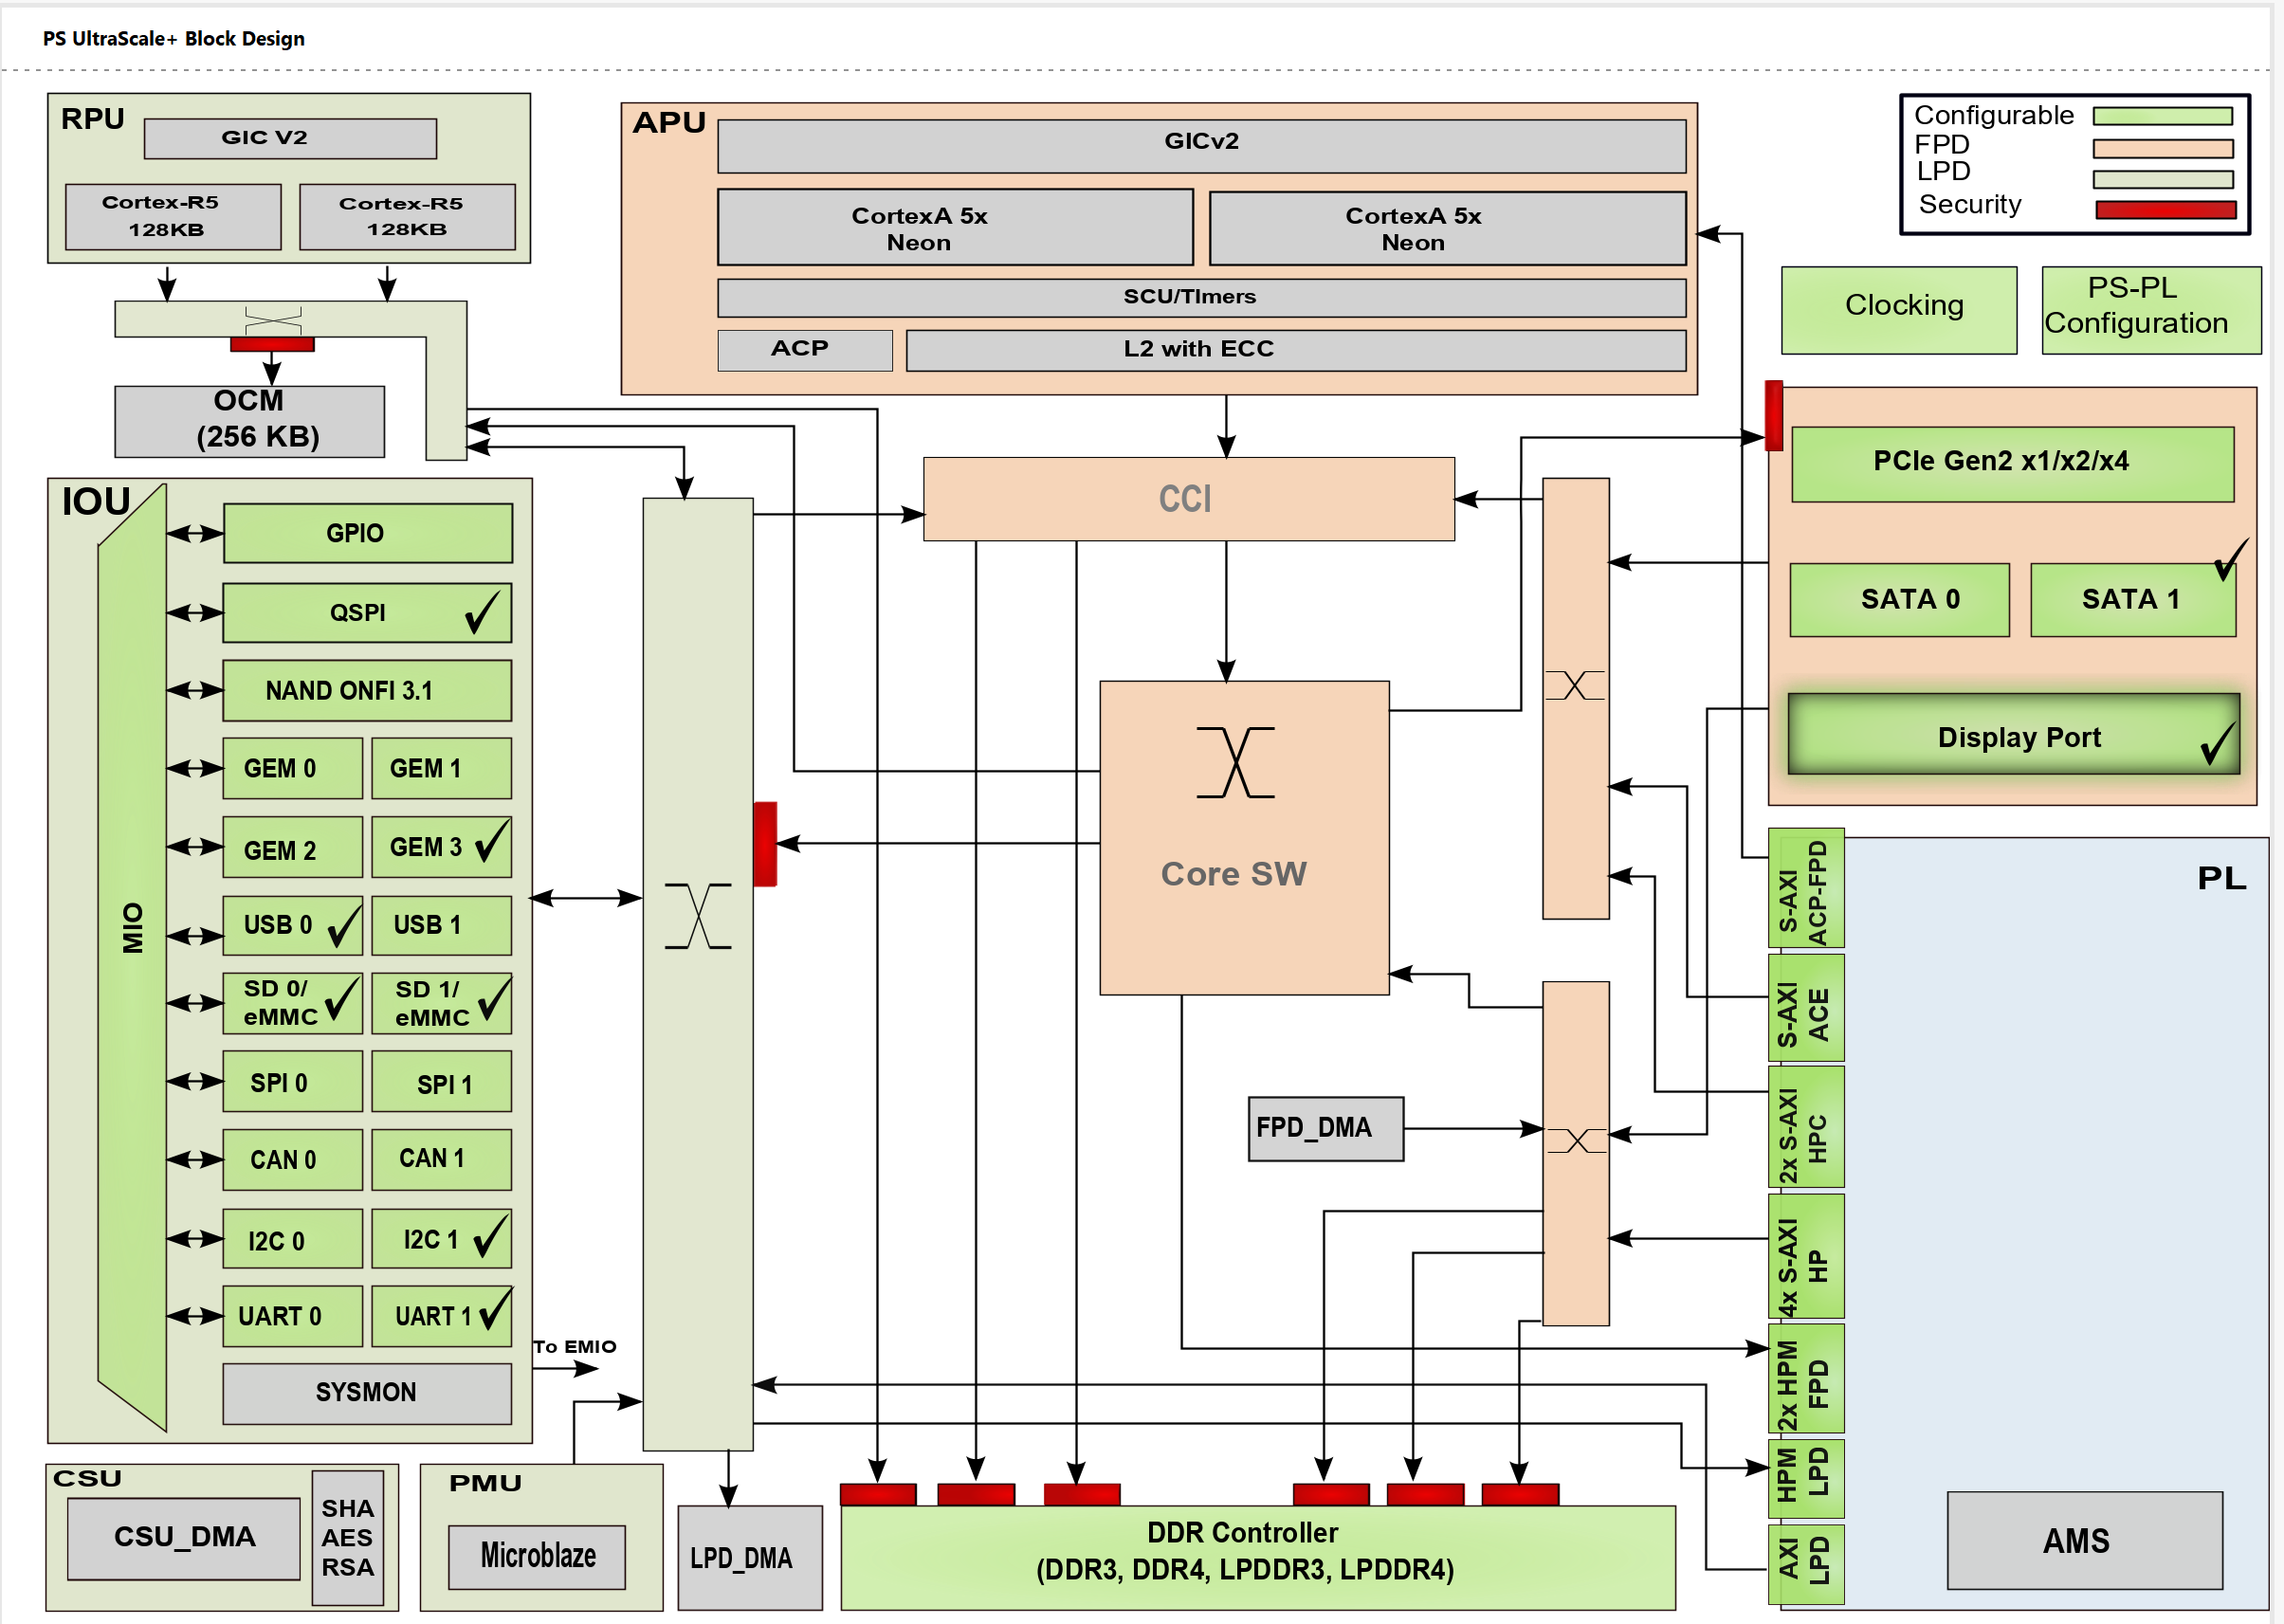
\includegraphics[width=0.8\textwidth]{USP_XMPUs}
    \caption [XMPU and XPPUs in a Zynq UltraScale+]{Xilinx Memory Protection Units (XMPUs) and Xilinx Peripheral Protection Units (XPPUs) within the Zynq UltraScale+ MPSoC architecture}
    \label{fig:XMPPUs}
\end{figure}

Unfortunately, this binary configuration is unsuitable for a multi-tenant configuration. Although there is a need for the supervisory mechanism (furnished by the CSP or the FPGA Vendor) to remain isolated from tenant components, there is also a need for isolation between different tenant components, a flexibility which is not afforded by TrustZone or its competitors. Instead, some form of more granular memory and peripheral isolation is required.

Many of the academic works that have been published on the topic of multi-tenant FPGA-based systems (such as those discussed in Section \ref{sec:LitImpl} have, at the least, acknowledged the need for memory isolation as a means of ensuring tenant data confidentiality and integrity. Unfortunately, many of these discussions are abstract in nature, and lack concrete implementation. For example, \cite{bag_cryptographically_2020} places the responsibility for memory isolation on the OpenStack architecture they base their design on, without a robust consideration of the application of this isolation to the programmable logic. Meanwhile, \cite{chen_enabling_2014} outlines a detailed plan for memory isolation, but does so by utilizing a processor based virtual environment for each partition, imposing appreciable system overhead while not guaranteeing isolation from malicious cotenants on the programmable logic.

As is evident from Figure \ref{fig:XMPPUs}, the XPPU and XMPU cores are used to enable the isolation of various key portions of the system, including the processors, IO, and various memory devices. However, it is important to note the absence of any isolation functionality within the programmable logic itself, which, tied with the practice of ``memory mapping'' various PL based logic devices, leaves an avenue for malicious co-tenants within the programmable logic to gain access to other tenants' IP. In \cite{noauthor_memory_2021}, Xilinx proposes the aforementioned XMPU-PL IP, which enables the previously absent isolation of memory-mapped PL devices at a granular level. A block diagram of this component is shown in Figure \ref{fig:XMPU_PL_BD}. Unfortunately, neither of these Xilinx references address the specific task of this effort, facilitating multiple mutually untrustworthy tenant on a single system. Rather, they propose a strict linear trust model that does not entertain the concept of multiple entities requiring equal but separate permissions.

\begin{figure}[h]
    \centering
    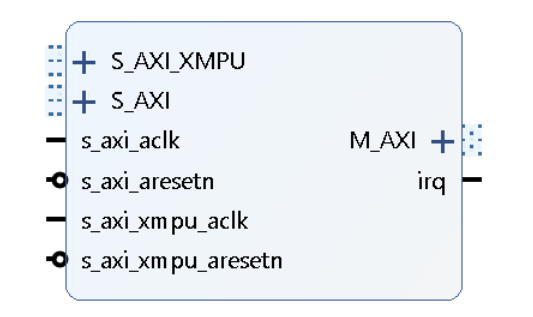
\includegraphics[width=0.5\textwidth]{XMPU_PL_Symbol}
    \caption [XMPU-PL IP Core]{Vivado Representation of the XMPU-PL IP \cite{noauthor_memory_2021}}
    \label{fig:XMPU_PL_Sym}
\end{figure}


%This work utilizes these XMPU-PL units to dynamically confine the decryption engines' memory access to whatever tenant partition they are currently processing encrypted bitstream data for (as determined by the scheduling engine outlined in Chapter \ref{ch:edfScheduling}). It also utilizes the XMPU-PLs to serve as a ``gate'' for all memory requests for each partition, thereby preventing a malicious actor from attempting to access other tenants' devices or memory space. By utilizing these XMPU-PL cores in an attestable bitstream (such as one provided by an FPGA vendor or trusted third party), the tenant can be assured of PL confidentiality and integrity.

The remainder of this chapter lays out a proposal to remedy this issue. First, it discusses the XMPU-PL core in detail, drawing heavily from reference designs presented in \cite{noauthor_memory_2021} and accompanying first-hand experimental results. Then, using a Trust-Zone based hierarchical separation between static components (such as the decryption engines), which form a portion of the bitstream provided from the trusted third party (FPGA vendor or independent trusted party), and tenant components withing their partition, the proposed design is able to ensure the integrity of the supervisory functions from a malicious tenant. Similarly, implementing XMPU-PL instances as a gateway for data flow into each tenant partition enables the partition to be strictly confined to its assigned memory space, and, additionally, allows the tenant to chose which peripherals to grant access to its partition. This last step is crucial to unlocking the full potential of FPGAs in a heterogenous environment, as they necessarily require interface with the other parts of the system in able to provide maximum usability.

\section{The XMPU-PL IP Core}

\begin{figure}[h]
    \centering
    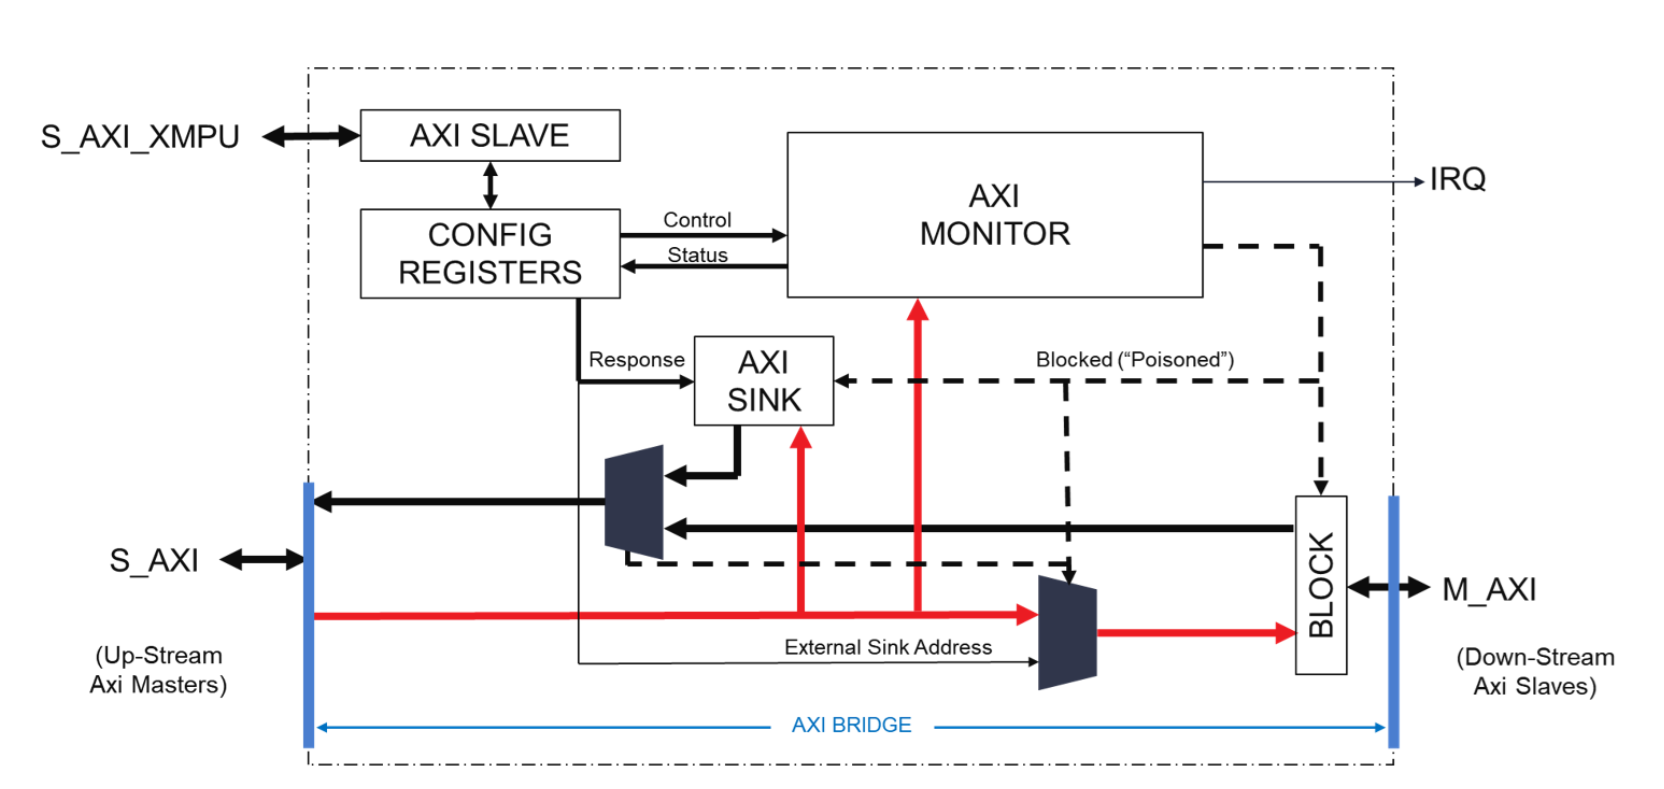
\includegraphics[width=0.8\textwidth]{XMPU_PLBlockDiagram}
    \caption [XMPU-PL Block Diagram]{Block diagram of the XMPU-PL IP \cite{noauthor_memory_2021}}
    \label{fig:XMPU_PL_BD}
\end{figure}

The XMPU-PL IP Core allows for the selective transit of AXI transactions from an Up-Stream AXI Master to Down-Stream AXI Slaves (as well as any responses flowing the other direction, i.e. data in response to a read request). The core extends the binary protection afforded by the TrustZone architecture by allowing address-restricted access to the AXI Slave Device. To achieve this, the core allows for the customization of up to 16 distinct regions of memory space, via the customization interface depicted in Figure \ref{fig:XMPU_region_config}. When configured, the XMPU-PL allows transactions to flow that are targeted at the given region if and only if the originating AXI Master is explicitly enabled in the ``Region XX Masters'' register. This register allows for the selective access of any of 32 distinct AXI Masters, including the various PS processors and interfaces. 

\begin{figure}[h]
    \centering
    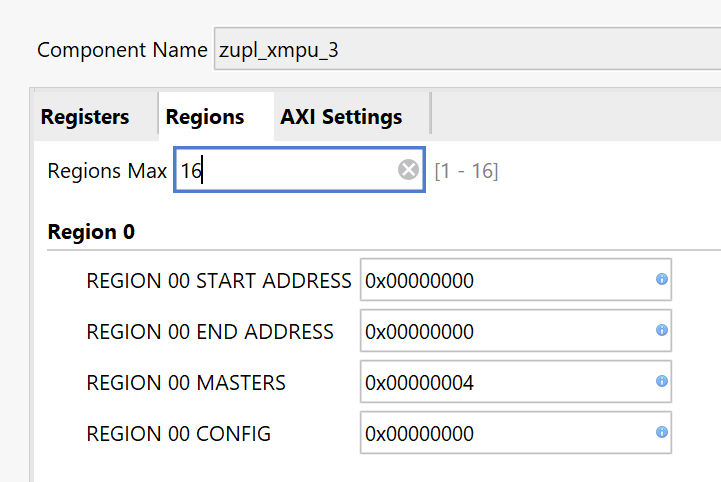
\includegraphics[width=0.5\textwidth]{XMPU_region_config}
    \caption[XMPU Region Configuration]{Configuration of the XMPU-PL IP}
    \label{fig:XMPU_region_config}
\end{figure}

In conjunction with address based filtering, each region can be configured with a TrustZone-based Secure or Non-Secure security level. By using this functionality, in conjunction with the ARM TrustZone based isolation of the trusted components from the untrusted, it is possible to completely restrict access to sensitive components, such as the decryption engines, to only those components that are explicitly enabled in the XMPU-PL. A full list of supported AXI Masters is presented in Appendix \ref{apx:axi-masters}.

Unfortunately, AXI Master-based verification only works against the specific AXI Masters pre-defined in the given register. This is due to an inherent design decision, whereby PL-based AXI Masters don't specify a Master ID in their transactions, making such differentiation impossible. Fortunately, the core can still be utilized as a combination of a TrustZone-based and memory region-based isolation mechanism in such an instance. This is done by modifying a pair of configuration parameters of the core, DefRdAllowed and DefWrAllowed, which control the behavior of the core when responding to requests that do not match any region defined in the region configuration registers. By setting these to their ``deny'' state, the core will deny all transactions that do not match any region defined in these registers, effectively preventing any access to memory regions that are not intended to be visible to the PL Master.

An additional feature afforded by the core is the ability to either statically or dynamically configure it. It is possible to provide design-time values to all of the registers utilized to control the core, and furthermore to lock those registers such that run-time modification is impossible. In this way, no additional setup overhead is required on the part of PS-based applications, and a malicious actor cannot compromise the integrity of the core by altering its isolation configuration. Alternatively, the registers can be exposed via a dedicated configuration AXI interface, enabling flexibility while also allowing only specific portions of the system to perform such updates.

Further register flags enable the implementer to customize the behavior of the core. For example, the response provided to an invalid request can be configured as one of several AXI status codes, ranging from an ``OK'' status to various error codes, some of which intentionally misrepresent the error as something other than a lack of permissions. Alternatively, such requests can be routed to a dedicated AXI Slave, such that custom responses can be provided. Additional registers allow for interrupt handling to allow for PS-PL communication.


\section{Isolation Lab Reference Designs}\label{sec:DMAIsolationLab}
The Xilinx document that proposes the XMPU-PL IP, \cite{noauthor_memory_2021}, includes a set of example ``Labs'', which enable the user to evaluate the functionality of the IP in an embedded environment. As part of this research effort, these designs, which were originally developed for the Xilinx ZCU102 development board, were modified for use on the AXU2CGB target specified in Section \ref{subsec:DMAEnvironmentHW}. This effort required a reconfiguration of the processor interface IP to account for the differing peripherals and memory controllers on the AXU2CGB target.

The tests provided by \cite{noauthor_memory_2021} provide tests of the XMPU-PL as part of a fully integrated isolated system. Such a system is configured via the processor interface IP's advanced configuration settings, as indicated in Figure \ref{fig:PS_int_isolation}. The reference design creates three partitions, one each for the Application Processor Unit (Cortex A processor cores), Real-Time Processor Unit (Cortex R processor cores), and the Power Management Unit (typically implemented as a MicroBlaze soft-processor, but not one that is user-generated). The design treats the PMU as the supervisory function of the system, with the RPU acting in a secured function while the APU performs untrusted functions.

\begin{figure}[h]
    \centering
    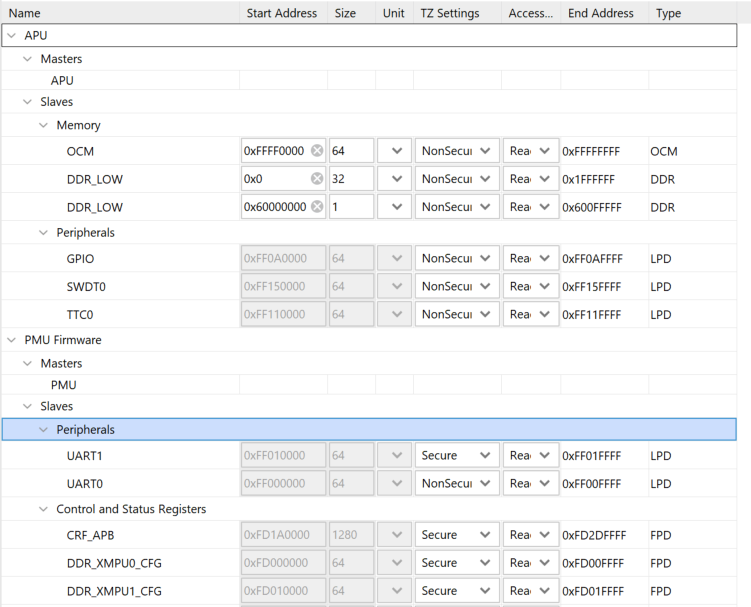
\includegraphics[width=0.8\textwidth]{PS_int_isolation}
    \caption{PS-PL Isolation Configuration}
    \label{fig:PS_int_isolation}
\end{figure}

\subsection{Lab Results}

In the example code accompanying \cite{noauthor_memory_2021}, Xilinx provides two sets of tests. Each utilizes the PMU as a supervisor, and both implement a First Stage Boot-loader (FSBL) on the RPU. However, one of the tests consists of attempts by the APU (which is non-secure), whereas the other exercises the XMPU (and other system components) from the RPU. As with the reference design itself, these tests required some modification in order to be run on the AXU2CGB target. Specifically, certain peripherals that are implemented on the larger ZCU102 target are not implemented on the AXU2CGB, and accordingly could not be integrated into the design (and accordingly, had to be removed from the test suite). 

Further modifications had to be made to account for the fact that the ZCU102 has a dual UART-over-USB interface that carries two serial channels, whereas the AXU2CGB only has one, which cannot be connected to the RPU subsystem due to design constraints. Fortunately, the target supports the transmission of a second UART over the JTAG interface, enabling monitoring of both the PMU in its supervisory role and the APU/RPU as they attempt to exercise it. Conversion of the JTAG interface on the AXU2CGB to a USB interface is accomplished using Alinx's ``USB Cable'', which, in keeping with the Xilinx device of the same name, is actually not a cable but instead its own complex PCB.

Using the two JTAG interfaces, one can view the results of attempts by the APU to compromise the secured PL components, as well as the PMU's response to these attempted violations. These results are captured in Figure \ref{fig:APU_Test_Suite}. As is shown in the figures, the APU is able to successfully access those memory regions (and memory-mapped devices) to which it is granted access (only a subset of which are shown for conciseness), but is unable to access the secure assets protected by the XMPU-PL core.

\begin{figure}[H]
    \centering
    \begin{subfigure}[b]{0.8\textwidth}
        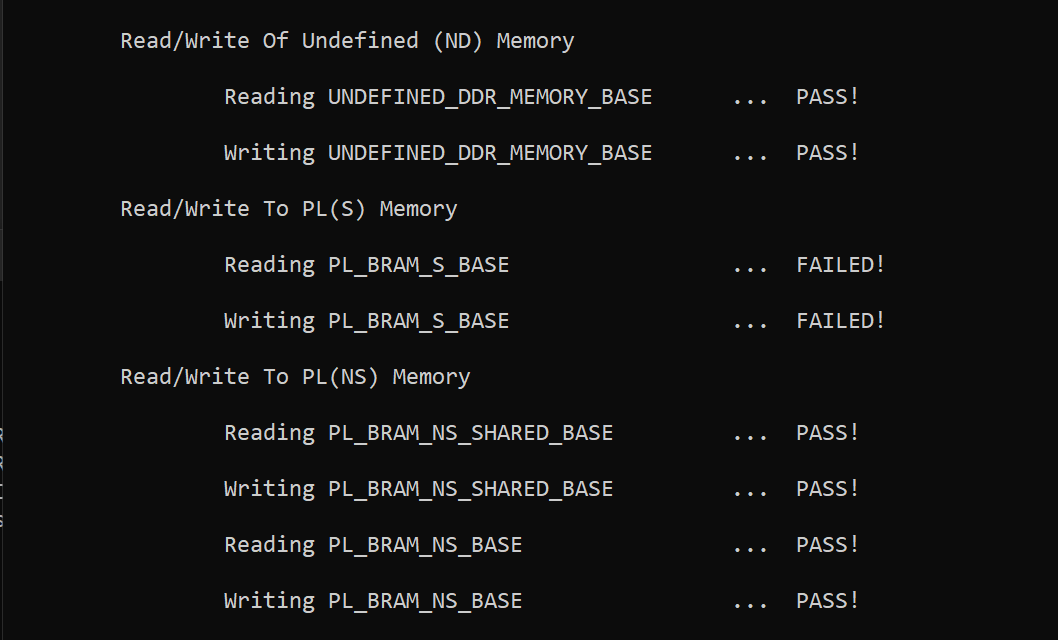
\includegraphics[width=\textwidth]{APU_FI/APU_PLReads}
        \caption{APU PL Read Attempt}
        \label{subfig:APU_PLRead}
    \end{subfigure}
\end{figure}
\begin{figure}[H]
    \ContinuedFloat
    \centering
    \begin{subfigure}[b]{0.8\textwidth}
        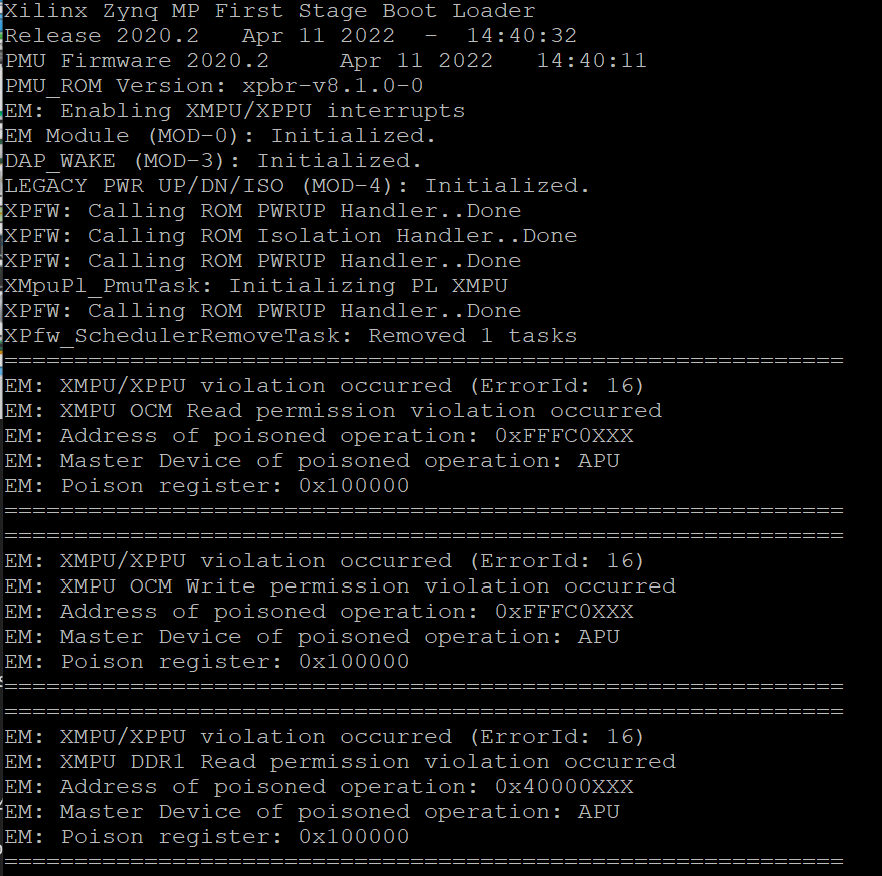
\includegraphics[width=\textwidth]{APU_FI/PMU}
        \caption{PMU Response to APU PL Read Attempt}
        \label{subfig:APU_PMU_Response}
    \end{subfigure}
    \caption{APU Test Suite}
    \label{fig:APU_Test_Suite}
\end{figure}

Meanwhile, the RPU is able to access those secure assets to which it was assigned, as well as the non-secure assets which were shared with it in the isolation configuration. It is also able to access the configuration registers of the XMPU-PL, which is functionality that was not permitted of the APU in its role as host to untrusted applications. These results are showcased in Figure \ref{fig:RPU_Test_Suite}. Specifically, note the lower portion of \ref{subfig:RPU_PLRead}, which showcases the value of the XMPU-PL's lock register as set to 1, preventing edits to the configuration registers by anything other than specific AXI Masters specified in the lock bypass register (including the RPU). The RPU then writes a 0 to this field to allow global edits, then reads the register back to verify that the value was set correctly.

\begin{figure}[H]
    \centering
    \begin{subfigure}[b]{0.8\textwidth}
        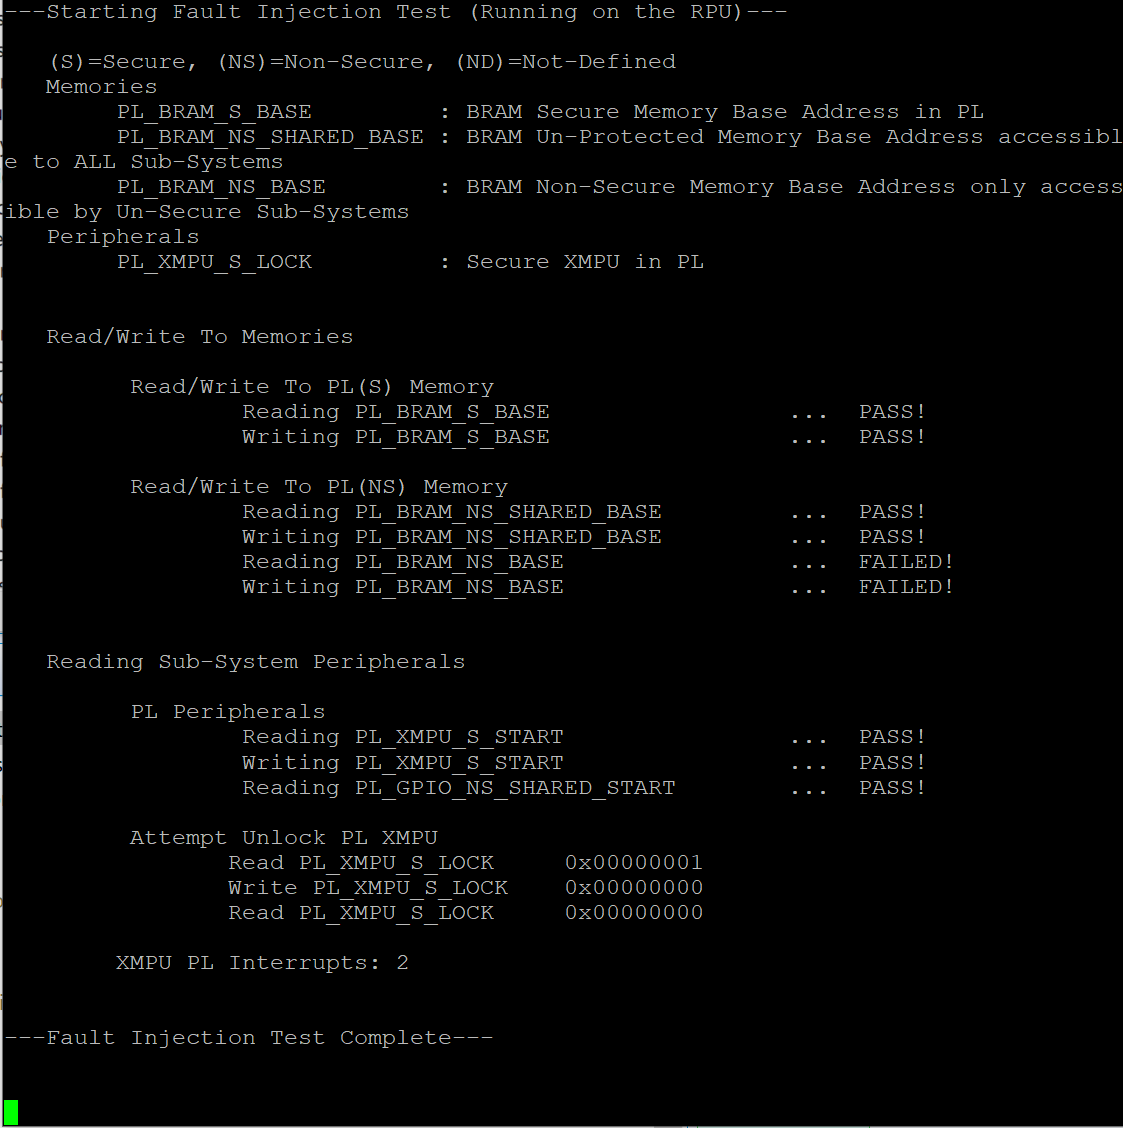
\includegraphics[width=\textwidth]{RPU_FI/RPU}
        \caption{RPU PL Read Attempt}
        \label{subfig:RPU_PLRead}
    \end{subfigure}
    \begin{subfigure}[b]{0.8\textwidth}
        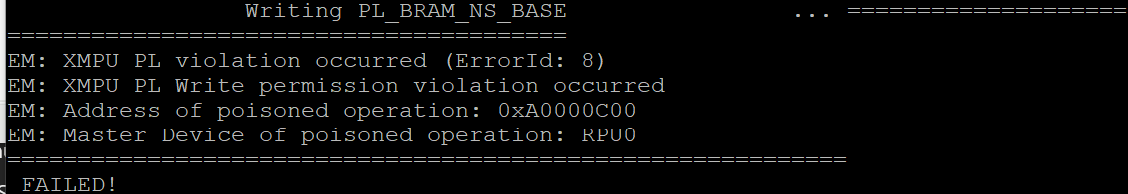
\includegraphics[width=\textwidth]{RPU_FI/PMU.png}
        \caption{PMU Response to RPU PL Read Attempt}
        \label{subfig:RPU_PMU_Response}
    \end{subfigure}
    \caption{RPU Test Suite}
    \label{fig:RPU_Test_Suite}
\end{figure}

\section{Proposed Memory Isolation Design}\label{sec:DMADesign}

The memory isolation scheme proposed by this research effort is depicted in Figure \ref{fig:XMPU-PLDesign}. As can be seen in the figure, the PL is laid out in a star-like design, with the processor interface (through which the various partitions are administered) at its core. Data from the processor interface is directed through an interconnect IP, which acts as a crossbar switch to route data to the appropriate target. From this interconnect, data flows through one of a series of XMPU-PL units, one per tenant partition, before entering a second interconnect from which data is distributed within the partition. In this way, data is free to flow between devices within a partition (over this internal interconnect), but all requests from external resources are constrained to trusted system components by the XMPU-PL. The configuration registers of this XMPU-PL are configured such that either the supervisory processes (the scheduler, etc.) or the tenant themselves (presumably through a configuration interface on the processor) can modify them. That way, the tenant can grant access to system peripherals that are needed for its operation, such as Ethernet interfaces, or allow certain PS devices access if desired.

Meanwhile, the static components (the AES and KAC cores, as well as the partial reconfiguration (DFX) controller) are similarly connected to XMPU-PL cores, but said cores are not configured in the same way as those restricting tenant components. As they are part of the trusted static partition, there is not a need for constraining the memory space these cores can access. However, there is a a need to restrict what portions of the system can access them - specifically, only the EDF Scheduler and its associated interfaces, as outlined in Chapter \ref{ch:edfScheduling}, have a legitimate need for these cores. 

Accordingly, this functionality would, in the comprehensive design, be located in an isolated execution environment, which could be granted ``Secure'' status within the TrustZone framework. By then constraining the decryption cores and the DFX Controller as secure resources, it is possible to prevent malicious access to these resources. To this end, the configuration registers of these cores are locked, and only trusted components (such as the Scheduler), can access them. Such access could be necessary in order to allow the Scheduler and its associated interfaces to alter the memory regions with which the AES core may interface, such as when it is reallocated to a new core.

Finally, an additional XMPU-PL is located downstream of the tenant partition, enabling restriction of the tenant's AXI Masters to solely those memory regions and peripherals to which it is entitled access (those allocated specifically to its partition). Like the XMPU-PL cores protecting the static components, the configuration registers of this core are locked, and the tenant has no capability to override these locks in an attempt to allow additional access. 

\begin{figure}[H]
    \centering
    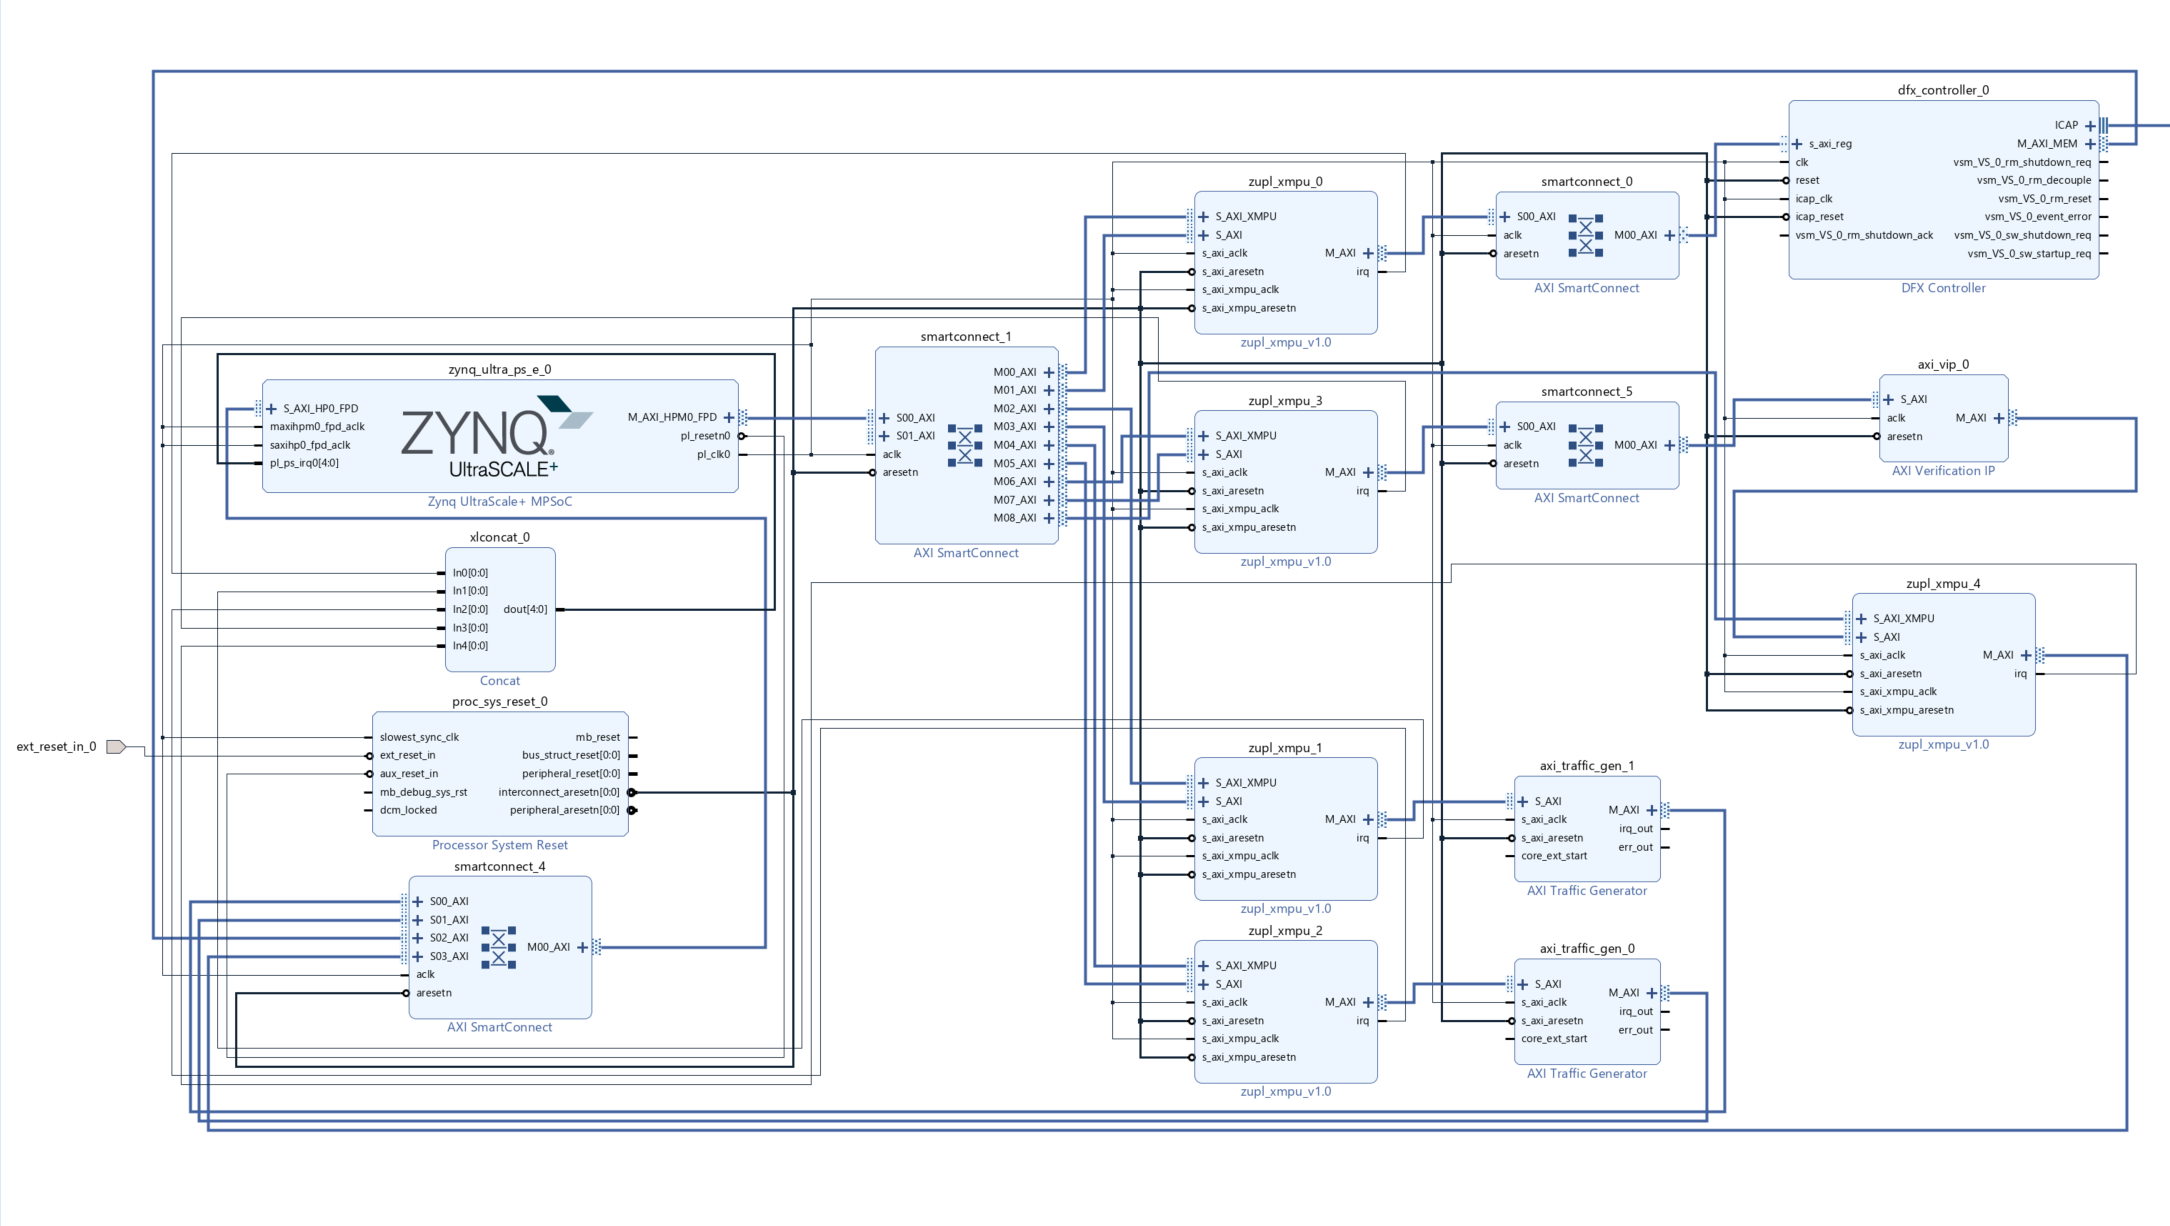
\includegraphics[width=.93\textheight, angle=90]{isolation_bd.png}
    \caption [Proposed XMPU-PL Design]{Xilinx Memory Protection Unit for Programmable Logic (XMPU-PL) in a Zynq UltraScale+ MPSoC architecture}
    \label{fig:XMPU-PLDesign}
\end{figure}

It should be acknowledged that the block diagram presented in Figure \ref{fig:XMPU-PLDesign} is necessarily simplified from what an actual CSP's implementation would afford. For starters, the design utilizes a pair of AXI Traffic Generator cores as stand-ins for a KAC engine and an AES engine, respectively. This is to enable a focus specifically on the memory isolation in this design, as opposed to attempting to implement a full architecture (and due to the lack of a licensed AES core, or any available KAC core in academia or industry). Additionally, it should be noted that this design only implements a single AES-representative core, and similarly only a single Dynamic Partial Reconfiguration Controller, where a more realistic implementation would include several AES engines (per the scheduler outlined in Chapter \ref{ch:edfScheduling}, above), as well as a separate Dynamic Partial Reconfiguration controller for each tenant partition. 

Similarly, the AXI Verification IP, located in the upper right portion of the diagram, is a stand-in for whatever user logic might be implemented in the tenant bitstream. This is the cause of the AXI Interconnect located adjacent to this IP, which seems extraneous given that it has only a single input and a single output. In reality, this IP would be located within the tenant partition, and would allow for various tenant devices to share the common entry point into the partition.

\subsection{Memory Regions in Proposed Design}\label{subsec:DMAMemRegions}
One of the key functions of the XMPU-PL is the ability to constrain upstream device access to specific regions of the overall memory map, thereby enabling isolation in excess of the traditional Secure/Non-secure binary dynamic. To take advantage of this functionality, the various XMPU-PL cores are configured with a variety of memory regions, which are divided at the system level in accordance with the table below. Note that these resources are at present constrained by the target hardware, which is discussed in detail in Section \ref{subsec:DMAEnvironmentHW}. These memory ranges are detailed in Table \ref{table:DMARanges}.

\begin{table}[ht!]
    \centering\begin{tabular}{|c|c|c|c|c|}
        \hline
        Region Purpose & Start Address & Width & Permitted Devices & Secure \\
        \hline
        PS Non-Secure Reserved & 0x00000000 & 1G & Sched/SM/Oth. PS & No \\
        PS Secure Reserved & 0x10000000 & 512M & Sched/SM/Oth. PS & Yes \\
        AES Key (Encrypted) & 0x90000000 & 64K & Sched/SM/KAC & Yes \\
        AES Key (Decrypted) & 0x90010000 & 64K & Sched/SM/KAC/AES & Yes \\
        Tenant Bitstream  (Encrypted) & 0x90020000 & 64M & Sched/SM/AES & Yes \\
        Tenant Bitstream  (Decrypted) & 0x94020000 & 64M & Sched/SM/AES/DFXC & Yes \\
        Tenant Storage & 0x98020000 & 128M & Tenant & No \\
        DFX Controller Config & 0xA0000000 & 64K & Sched/SM & Yes \\
        DFXC XMPU-PL Config & 0xA0010000 & 64K & Sched/SM & Yes \\
        AES XMPU-PL Config & 0xA0020000 & 64K  &Sched/SM & Yes \\
        KAC XMPU-PL Config & 0xA0030000 & 64K & Sched/SM & Yes \\
        KAC Engine Config & 0xA0040000 & 64K & Sched/SM & Yes \\
        AES Engine Config & 0xA0050000 & 64K & Sched/SM & Yes \\
        Tenant XMPU-PL Config (US) & 0xA0060000 & 64K & Sched/SM/Tenant & No \\
        Tenant XMPU-PL Config (DS) & 0xA0070000 & 64K & Sched/SM & No \\
        \hline
    \end{tabular}
    \caption{Memory Ranges in the Isolation Design}
    \label{table:DMARanges}
\end{table}

It should be noted that several of these ranges are appreciably larger than are needed, especially for configuration register spaces with a countably small number of registers. In these cases, these address ranges were assigned out of convenience of numerical value, as well as to allow for flexibility should future iterations of those components require additional register space. Such spaces could certainly be optimized should more space be required in a final design.

\section{Development and Test Environment}\label{sec:DMAEnvironment}

\subsection{Development Environment}\label{subsec:DMAEnvironmentDev}
The design presented in \ref{fig:XMPU-PLDesign} was implemented utilizing the same developer machine as outlined in \ref{subsec:devEnv}. Specifically, the development machine used by the authors in the course of this project was a Windows 10 Professional Edition 64-bit laptop featuring an Intel Core i7-9750H CPU with a base frequency of 2.60GHz. The machine featured 16 GB of DDR4 DRAM and a 1 TB SSD. Furthermore, the build process utilized the same Docker container as outlined in \ref{subsec:devEnv} to facilitate the development of the design.

\subsection{Target Hardware}\label{subsec:DMAEnvironmentHW}
Unlike the previous design, the desired use of the UltraScale+ architecture, with all of the isolation benefits outlined above, required the transition of the research effort away from the use of the ZedBoard as a hardware platform of choice. Instead, this effort targeted a recently released development platform that provides an affordable UltraScale+ MPSoC system, the Alinx AXU2CGB. The AXU2CGB, depicted in Figure \ref{fig:AXU2CGB}, is a compact development platform that includes an XCZU2CG-1SFVC784E UltraScale+ MPSoC. This MPSoC integrates a Dual-Core ARM Cortex-A53 Application Processor with a Dual-Core ARM Cortex-R5 Real Time Processor, combined with an FPGA that boasts over 103,000 logic cells, 94,000 look up tables, 240 DSP slices, 5.3 Mb of Block RAM, and 32MB of QSPI Flash. The larger AXU2CGB board also provides 2 GB of DDR4 RAM, as well as an 8GB EMMC Flash device.

\begin{figure}
    \centering
    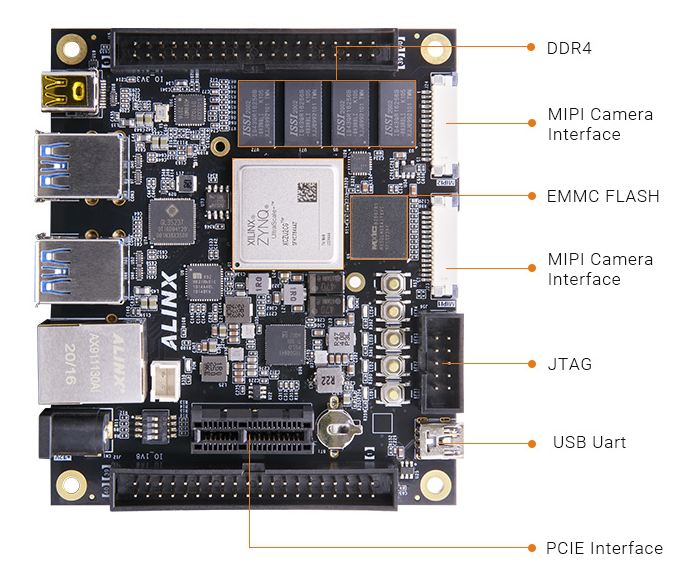
\includegraphics[]{axu2cgb.png}
    \caption[AXU2CGB Development System]{Alinx AXU2CGB Development System, with key components highlighted \cite{noauthor_axu2cgb_nodate}}
    \label{fig:AXU2CGB}
\end{figure}

\subsection{Target Operating System}\label{subsec:DMAEnvironmentOS}
Although the integration of the architecture depicted in Figure \ref{fig:XMPU-PLDesign} into a larger system integrating the PS-based scheduler outlined in Chapter \ref{ch:edfScheduling} would necessitate a PetaLinux (or similar) environment, the isolated development of this functionality as outlined in this section does not strictly necessitate a full-featured operating system be implemented for its verification. Furthermore, the XMPU-PL was not presented by Xilinx with accompanying Linux-compatible drivers, which necessarily differ from those used in a ``Standalone'' configuration. To this end, this effort chose to implement and exercise this design in such a standalone environment. 

Care should be taken in applying the phrase ``Standalone'' to this design. In a traditional sense, this would indicate that the target application (in this case, test software to exercise the XMPU-PL) is compiled directly to ARM instructions, which execute immediately following the application of power to the system. However, the MPSoC is sufficiently complex that such an assumption would be unwieldy. To this end, what Xilinx calls a ``Standalone'' project is actually a project that utilizes its Standalone library, which it describes as ``a single-threaded, simple operating system (OS) platform that provides the lowest layer of software modules used to access processor-specific functions'' \cite{noauthor_os_2020}.
% Much like the ZedBoard, the AXU2CGB is well suited for the PetaLinux operating environment provided by Xilinx for use on its SoCs. Initial efforts targeting this board have utilized the stock PetaLinux image provided with the purchase of the board, which is based on the same PetaLinux 2020.2 toolchain as previously discussed. Later efforts implementing various test applications have utilized slightly modified variants, which are discussed in subsequent sections. Additionally, certain tests were conducted in a ``bare-metal'' environment, wherein the applications were executed directly on the target without an operating system serving as a middle layer.

\section{Implementation Results}\label{sec:DMAResults}

The direct experimental results of the implementation of the architecture outlined in Figure \ref{fig:XMPU-PLDesign}, above, consist of serial interface printouts that very nearly mirror Figures \ref{fig:APU_Test_Suite} and \ref{fig:RPU_Test_Suite}, above. Accordingly, they are not included herein for purposes of brevity. However, one immediate takeaway from the implementation of the design shown in Figure \ref{fig:XMPU-PLDesign}, above, is that it consumes a large portion of the available PL, even on a recent (and comparatively large) FPGA such as the one afforded by the AXU2CGB. As the utilization report shown in Figure \ref{fig:XMPU-PLUtilization} shows, nearly 95\% of all Look Up Tables (LUTs) are consumed in this design. However, it should be noted that such an FPGA is appreciably smaller still than the large format devices that will likely become the tool of choice for cloud based operations, and in such instances this design yields appreciable savings over the previously proposed architectures. Furthermore, a portion of this utilization is consumed by the AXI Traffic Generator IPs acting as stand-ins for the KAC and AES engines, as well as for the verification IP standing in for the user logic. The resources consumed by these cores should not be taken as representative of the actual IP they are intended to act as a substitute for.

\begin{figure}
    \centering
    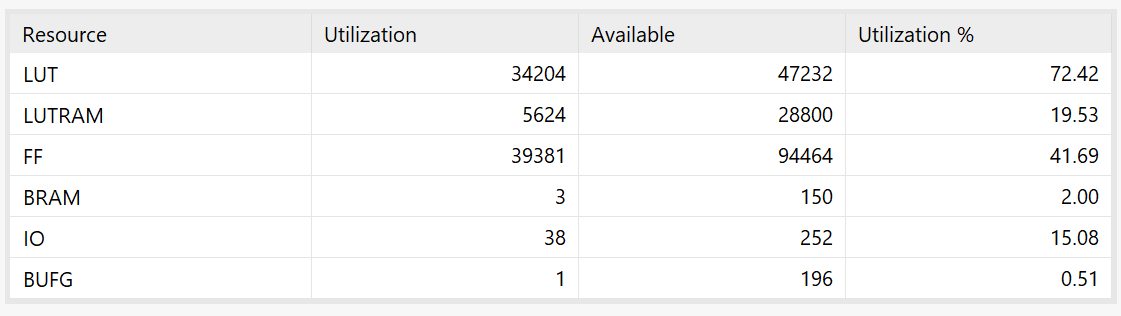
\includegraphics[width=0.5\textwidth]{xmpupl_utilization.png}
    \caption[Memory Isolation Resource Utilization]{Resource Utilization for the XMPU-PL design, as implemented on the AXU2CGB}
    \label{fig:XMPU-PLUtilization}
\end{figure}

Furthermore, it should be noted that the current implementation of the design still utilizes the isolation architecture implemented in the reference designs, wherein the PMU acts in the supervisory capacity, detecting rejected transactions from the PL. In the context of the larger reference design, it is likely that this functionality would be located within one of the hard processing systems, likely within the APU as the security monitor functionality would likely require multithreading, a function not afforded by the MMU-less Cortex-R5 cores. As was discussed earlier in this chapter, such a migration would require the implementation of custom Linux drivers for the IP, as it is currently provided with drivers only for the standalone environment.               % INCLUDE: DMA Protection
% !TeX root = ../SDonchezThesis.tex

\chapter{Conclusion}\label{ch:conclusion}                  % INCLUDE: conclusion

\addcontentsline{toc}{chapter}{References} 

\bibliographystyle{ECE_ReportTemplate/IEEEbib}
\bibliography{SDonchezResearch}

%appendices
% !TeX root = ../SDonchezThesis.tex

\appendix

\chapter{EDF Development Container Specification}\label{apx:EDFDocker}
\begin{lstlisting}[language=docker, breaklines=true, caption={Dockerfile for EDF Development Container}, label=lst:Dockerfile]
FROM ubuntu:18.04

# build with "docker build --build-arg PETA_VERSION=2020.2 --build-arg PETA_RUN_FILE=petalinux-v2020.2-final-installer.run -t petalinux:2020.2 ."

# install dependences:

ARG UBUNTU_MIRROR
RUN [ -z "${UBUNTU_MIRROR}" ] || sed -i.bak s/archive.ubuntu.com/${UBUNTU_MIRROR}/g /etc/apt/sources.list 

RUN apt-get update &&  DEBIAN_FRONTEND=noninteractive apt-get install -y -q \
  build-essential \
  sudo \
  tofrodos \
  iproute2 \
  gawk \
  net-tools \
  expect \
  libncurses5-dev \
  update-inetd \
  libssl-dev \
  flex \
  bison \
  libselinux1 \
  gnupg \
  wget \
  socat \
  gcc-multilib \
  libidn11 \
  libsdl1.2-dev \
  libglib2.0-dev \
  lib32z1-dev \
  libgtk2.0-0 \
  libtinfo5 \
  xxd \
  screen \
  pax \
  diffstat \
  xvfb \
  xterm \
  texinfo \
  gzip \
  unzip \
  cpio \
  chrpath \
  autoconf \
  lsb-release \
  libtool \
  libtool-bin \
  locales \
  kmod \
  git \
  rsync \
  bc \
  u-boot-tools \
  python \
  xinetd \
  tftpd \
  tftp \
  libsm6 \
  libxi6 \
  libxrandr2 \
  libfreetype6 \
  libfontconfig \
  libswt-gtk-4-java \
 && apt-get clean \
 && rm -rf /var/lib/apt/lists/*

RUN dpkg --add-architecture i386 &&  apt-get update &&  \
      DEBIAN_FRONTEND=noninteractive apt-get install -y -q \
      zlib1g:i386 \
    && apt-get clean \
    && rm -rf /var/lib/apt/lists/*

ARG PETA_RUN_FILE
ARG VIVADO_TAR_FILE
ARG VIVADO_VERSION

RUN locale-gen en_US.UTF-8 && update-locale

#make a Vivado user
RUN adduser --disabled-password --gecos '' vivado && \
  usermod -aG sudo vivado && \
  echo "vivado ALL=(ALL) NOPASSWD: ALL" >> /etc/sudoers

COPY .devcontainer/accept-eula.sh /tmp/
COPY .devcontainer/${VIVADO_TAR_FILE}.tar.gz /
COPY .devcontainer/install_config_vitis.txt /
COPY .devcontainer/install_config_petalinux.txt /

#config tftp server
COPY .devcontainer/tftp.in /etc/xinetd.d/tftp
RUN mkdir /tftpboot
RUN chmod ugo+rw /tftpboot/
RUN service xinetd stop
RUN service xinetd start

# run the install

RUN echo "Extracting Vivado tar file" 
RUN tar xzf ${VIVADO_TAR_FILE}.tar.gz 
RUN rm ${VIVADO_TAR_FILE}.tar.gz
RUN ${VIVADO_TAR_FILE}/xsetup --agree 3rdPartyEULA,WebTalkTerms,XilinxEULA --batch Install --config install_config_vitis.txt 
RUN ${VIVADO_TAR_FILE}/xsetup --agree 3rdPartyEULA,WebTalkTerms,XilinxEULA --batch Install --config install_config_petalinux.txt
RUN mkdir /tools/Xilinx/PetaLinux/${VIVADO_VERSION}/install/
RUN chmod -R 777 /tools/Xilinx/PetaLinux/${VIVADO_VERSION}/
RUN chmod -R 777 /tmp/
RUN cd /tmp && \
  sudo -u vivado -i /tmp/accept-eula.sh /tools/Xilinx/PetaLinux/${VIVADO_VERSION}/bin/${PETA_RUN_FILE} /tools/Xilinx/PetaLinux/${VIVADO_VERSION}/install/
RUN rm -f /tools/Xilinx/PetaLinux/${VIVADO_VERSION}/bin/${PETA_RUN_FILE} /tmp/accept-eula.sh
RUN rm -rf ${VIVADO_TAR_FILE}*

# make /bin/sh symlink to bash instead of dash:
RUN echo "dash dash/sh boolean false" | debconf-set-selections
RUN DEBIAN_FRONTEND=noninteractive dpkg-reconfigure dash

USER vivado
ENV HOME /home/vivado
ENV LANG en_US.UTF-8

#add vivado tools to path
RUN echo "service xinetd start" >> /home/vivado/.bashrc
RUN echo "source /tools/Xilinx/Vitis/2020.2/settings64.sh" >> /home/vivado/.bashrc
RUN echo "source /tools/Xilinx/PetaLinux/2020.2/install/settings.sh" >> /home/vivado/.bashrc

#setup vivado license
RUN mkdir /home/vivado/.Xilinx
COPY .devcontainer/Xilinx.lic /home/vivado/.Xilinx/
\end{lstlisting}

\chapter{AXI Masters Supported by the XMPU-PL IP Core}\label{apx:axi-masters}
The table below indicates the various AXI masters supported by the XMPU-PL IP core. These masters are supported in both the lock bypass (for XMPU-PL configuration) and AXI Master-based region restriction registers. This table is recreated from \cite{noauthor_memory_2021}.

\begin{table}[ht!]
  \centering\begin{tabular}{|c|c|c|c|l|}
      \hline
      Field Name & Bits & Type & Reset Value & \multicolumn{1}{c|}{Description} \\
      \hline
      Reserved & 31 & ro & 0x0 & Reserved \\
      MID\_FPD\_DMA[6:7] & 30 & rw & 0x0 & Enable FPD DMA [ch 6:7] \\
      MID\_FPD\_DMA[4:5] & 29 & rw & 0x0 & Enable FPD DMA [ch 4:5] \\
      MID\_FPD\_DMA[2:3] & 28 & rw & 0x0 & Enable FPD DMA [ch 2:3] \\
      MID\_FPD\_DMA[0:1] & 27 & rw & 0x0 & Enable FPD DMA [ch 0:1] \\
      MID\_DP\_DMA[4:5] & 26 & rw & 0x0 & Enable DisplayPort DMA [ch 4:5] \\
      MID\_DP\_DMA[2:3] & 25 & rw & 0x0 & Enable DisplayPort DMA [ch 2:3] \\
      MID\_DP\_DMA[0:1] & 24 & rw & 0x0 & Enable DisplayPort DMA [ch 0:1] \\
      MID\_PCIE & 23 & rw & 0x0 & Enable PCIe \\
      MID\_DAP\_AXI & 22 & rw & 0x0 & Enable Debug Access Port AXI \\
      MID\_GPU & 21 & rw & 0x0 & Enable GPU \\
      MID\_SATA1 & 20 & rw & 0x0 & Enable SATA1 \\
      MID\_SATA0 & 19 & rw & 0x0 & Enable SATA0 \\
      MID\_APU & 18 & rw & 0x0 & 
        \begin{tabular}{@{}l@{}}
          Enable APU \\ 
           \quad\textit{\textbf{Note}}: Requires that AxProt[1]=0. 
        \end{tabular}  
        \\
      MID\_GEM3 & 17 & rw & 0x0 & Enable GEM3 \\
      MID\_GEM2 & 16 & rw & 0x0 & Enable GEM2 \\
      MID\_GEM1 & 15 & rw & 0x0 & Enable GEM1 \\
      MID\_GEM0 & 14 & rw & 0x0 & Enable GEM0 \\
      MID\_QSPI & 13 & rw & 0x0 & Enable QSPI \\
      MID\_NAND & 12 & rw & 0x0 & Enable NAND \\
      MID\_SD1 & 11 & rw & 0x0 & Enable SD1 \\
      MID\_SD0 & 10 & rw & 0x0 & Enable SD0 \\
      MID\_LPD\_DMA[6:7] & 9 & rw & 0x0 & Enable LPD DMA [ch 6:7] \\
      MID\_LPD\_DMA[4:5] & 8 & rw & 0x0 & Enable LPD DMA [ch 4:5] \\
      MID\_LPD\_DMA[2:3] & 7 & rw & 0x0 & Enable LPD DMA [ch 2:3] \\
      MID\_LPD\_DMA[0:1] & 6 & rw & 0x0 & Enable LPD DMA [ch 0:1] \\
      MID\_DAP\_APB & 5 & rw & 0x0 & Enable Debug Access Port APB \\
      MID\_USB1 & 4 & rw & 0x0 & Enable USB1 \\
      MID\_USB0 & 3 & rw & 0x0 & Enable USB0 \\
      MID\_PMU & 2 & rw & 0x1 & Enable PMU \\
      MID\_RPU1 & 1 & rw & 0x0 & Enable RPU1 \\
      MID\_RPU0 & 0 & rw & 0x0 & Enable RPU0 \\
      \hline
  \end{tabular}
  \caption{Memory Ranges in the Isolation Design}
  \label{table:XMPU_PL_AXI_Masters}
\end{table}
\end{document}                              % The required last line